% ------------------------------------------------------------------------
% ------------------------------------------------------------------------
% Modelo para Trabalhos Academicos utilizando a classe abntex2
%
%  Adaptado de UFSC para IFFar
% ------------------------------------------------------------------------
% ------------------------------------------------------------------------

\documentclass[
	% -- opções da classe memoir --
	12pt,				% tamanho da fonte
	%openright,			% capítulos começam em pág ímpar (insere página vazia caso preciso)
	oneside,			% para impressão no anverso. Oposto a twoside
	a4paper,			% tamanho do papel. 
	% -- opções da classe abntex2 --
	chapter=TITLE,		% títulos de capítulos convertidos em letras maiúsculas
	section=TITLE,		% títulos de seções convertidos em letras maiúsculas
	%subsection=TITLE,	% títulos de subseções convertidos em letras maiúsculas
	%subsubsection=TITLE,% títulos de subsubseções convertidos em letras maiúsculas
	% -- opções do pacote babel --
	english,			% idioma adicional para hifenização
	%french,				% idioma adicional para hifenização
	%spanish,			% idioma adicional para hifenização
	brazil				% o último idioma é o principal do documento
	]{abntex2}

\usepackage{setup/ufscthesisA4-alf}
\usepackage{float}
\usepackage{tikz}                % fluxogramas compilados no próprio documento
\usetikzlibrary{positioning,arrows.meta,fit}

% ---
% Filtering and Mapping Bibliographies
% ---
% Pacotes de citações
% ---
\usepackage{csquotes}
\usepackage[backend = biber, style = abnt]{biblatex}
% \citeonline pertence ao abntex2cite. Neste modelo o estilo é biblatex-abnt, e o equivalente é \textcite.
\newcommand{\citeonline}{\textcite}
% FIXME Se desejar estilo numérico de citações,  comente a linha acima e descomente a linha a seguir.
% \usepackage[backend = biber, style = numeric-comp]{biblatex}

\setlength\bibitemsep{\baselineskip}
\DeclareFieldFormat{url}{Disponível~em:\addspace\url{#1}}
\NewBibliographyString{sineloco}
\NewBibliographyString{sinenomine}
\DefineBibliographyStrings{brazil}{%
	sineloco     = {\mkbibemph{S\adddot l\adddot}},
	sinenomine   = {\mkbibemph{s\adddot n\adddot}},
	andothers    = {\mkbibemph{et\addabbrvspace al\adddot}},
	in			 = {\mkbibemph{In:}}
}

\addbibresource{aftertext/references.bib} % Seus arquivos de referências

% ---
\DeclareSourcemap{
	\maps[datatype=bibtex]{
		% remove fields that are always useless
		\map{
			\step[fieldset=abstract, null]
			\step[fieldset=pagetotal, null]
		}
		% remove URLs for types that are primarily printed
%		\map{
%			\pernottype{software}
%			\pernottype{online}
%			\pernottype{report}
%			\pernottype{techreport}
%			\pernottype{standard}
%			\pernottype{manual}
%			\pernottype{misc}
%			\step[fieldset=url, null]
%			\step[fieldset=urldate, null]
%		}
		\map{
			\pertype{inproceedings}
			% remove mostly redundant conference information
			\step[fieldset=venue, null]
			\step[fieldset=eventdate, null]
			\step[fieldset=eventtitle, null]
			% do not show ISBN for proceedings
			\step[fieldset=isbn, null]
			% Citavi bug
			\step[fieldset=volume, null]
		}
	}
}
% ---

% ---
% Informações de dados para CAPA e FOLHA DE ROSTO
% ---
% FIXME Substituir 'Nome completo do autor' pelo seu nome.
\autor{Lorenzo de Ávila Carpes}
% FIXME Substituir 'Título do trabalho' pelo título da trabalho.
\titulo{Modelo de triagem para identificação de risco metabólico associado ao Diabetes Mellitus tipo 2 utilizando variáveis não invasivas dos microdados da Subamostra Laboratorial da Pesquisa Nacional de Saúde (PNS 2013)}
% FIXME Substituir 'Subtítulo (se houver)' pelo subtítulo da trabalho.  
% Caso não tenha substítulo, comente a linha a seguir.
% \subtitulo{}
% FIXME Substituir 'XXXXXX' pelo nome do seu
% orientador.

\orientador{Icaro Lins Iglesias}
% FIXME Se for orientado por uma mulher, comente a linha acima e descomente a linha a seguir.
% \orientador[Orientadora]{Nome da orientadora, Dra.}
% FIXME Substituir 'XXXXXX' pelo nome do seu
% coorientador. Caso não tenha coorientador, comente a linha a seguir.
% \coorientador{Prof. XXXXXX, Dr.}
% FIXME Se for coorientado por uma mulher, comente a linha acima e descomente a linha a seguir.
% \coorientador[Coorientadora]{XXXXXX, Dra.}
% FIXME Substituir 'XXXXXX' pelo nome do Coordenador do 
% programa/curso.
\coordenador{Prof. Claiton Marques Corrêa, Dr.}
% FIXME Se for coordenadora mulher, comente a linha acima e descomente a linha a seguir.
% \coordenador[Coordenadora]{Nome da Coordenadora, Dra.}
% FIXME Substituir '[ano da entrega]' pelo ano (ano) em que seu trabalho foi defendido.
\ano{2026}
% FIXME Substituir '[dia] de [mês] de [ano]' pela data em que ocorreu sua defesa.
\data{[dia] de [mês] de [ano]}
% FIXME Substituir '[Cidade da defesa]' pela cidade em que ocorreu sua defesa.
\local{São Borja, RS}
\instituicaosigla{IFFar}
\instituicao{Instituto Federal de Educação, Ciência e Tecnologia Farroupilha}
% FIXME Substituir 'Dissertação/Tese' pelo tipo de trabalho (Tese, Dissertação). 
\tipotrabalho{Trabalho de Conclusão de Curso}
% FIXME Substituir '[licenciado/bacharel] em [nome do título obtido]' pela grau adequado.
\formacao{Bacharel em Sistemas de Informação}
% FIXME Substituir '[licenciado/bacharel]' pelo nivel adequado.
\nivel{Bacharel}
% FIXME Substituir 'Curso de Graduação em [XXXXXXXX]' pela curso adequado.
\programa{Bacharelado em Sistemas de Informação}
% FIXME Substituir 'Campus XXXXXX ou Centro de XXXXXX' pelo campus ou centro adequado.
\centro{Campus São Borja}
\preambulo
{%
\imprimirtipotrabalho~apresentado~como~requisito~parcial~para~a~obtenção~do~título~de~\imprimirformacao~no~\imprimircentro~do~\imprimirinstituicao.
}
% ---

% ---
% Configurações de aparência do PDF final
% ---
% alterando o aspecto da cor azul
\definecolor{blue}{RGB}{41,5,195}
% informações do PDF
\makeatletter
\hypersetup{
     	%pagebackref=true,
		pdftitle={\@title}, 
		pdfauthor={\@author},
    	pdfsubject={\imprimirpreambulo},
	    pdfcreator={LaTeX with abnTeX2},
		pdfkeywords={diabetes mellitus tipo 2, aprendizado de máquina, PNS 2013, triagem, SHAP}, 
		colorlinks=true,       		% false: boxed links; true: colored links
    	linkcolor=black,%blue,          	% color of internal links
    	citecolor=black,%blue,        		% color of links to bibliography
    	filecolor=black,%magenta,      		% color of file links
		urlcolor=black,%blue,
		bookmarksdepth=4
}
\makeatother
% ---

% ---
% compila a lista de abreviaturas e siglas e a lista de símbolos
% ---

% Declaração das siglas
\siglalista{APS}{Atenção Primária à Saúde}
\siglalista{AUC-ROC}{Área sob a Curva ROC}
\siglalista{CC}{Circunferência da Cintura}
\siglalista{CEP}{Comitê de Ética em Pesquisa}
\siglalista{CNS}{Conselho Nacional de Saúde}
\siglalista{CRISP-DM}{\textit{Cross Industry Standard Process for Data Mining}}
\siglalista{DM}{Diabetes Mellitus}
\siglalista{DM2}{Diabetes Mellitus tipo 2}
\siglalista{ELSA-Brasil}{Estudo Longitudinal de Saúde do Adulto}
\siglalista{FINDRISC}{\textit{Finnish Diabetes Risk Score}}
\siglalista{HAS}{Hipertensão Arterial Sistêmica}
\siglalista{HbA1c}{Hemoglobina Glicada}
\siglalista{IBGE}{Instituto Brasileiro de Geografia e Estatística}
\siglalista{IMC}{Índice de Massa Corporal}
\siglalista{KNN}{\textit{K-Nearest Neighbors}}
\siglalista{ML}{\textit{Machine Learning}}
\siglalista{NNS}{Número Necessário para Rastrear}
\siglalista{PEC}{Prontuário Eletrônico do Cidadão}
\siglalista{PNS}{Pesquisa Nacional de Saúde}
\siglalista{PR-AUC}{Área sob a Curva de Precisão e Sensibilidade}
\siglalista{RCEst}{Razão Cintura-Estatura}
\siglalista{SHAP}{\textit{SHapley Additive exPlanations}}
\siglalista{SIGTAP}{Sistema de Gerenciamento da Tabela de Procedimentos, Medicamentos e OPM do SUS}
\siglalista{SIPD}{Sistema Integrado de Pesquisas Domiciliares}
\siglalista{SISAB}{Sistema de Informação em Saúde para a Atenção Básica}
\siglalista{SMOTE}{\textit{Synthetic Minority Over-sampling Technique}}
\siglalista{SRH}{\textit{Self-Rated Health}}
\siglalista{SUS}{Sistema Único de Saúde}
\siglalista{VIF}{Fator de Inflação de Variância}
\siglalista{XAI}{Inteligência Artificial Explicável}

% Declaração dos simbolos
% O trabalho não usa símbolos próprios; a lista de símbolos está desativada no pré-texto.

% compila a lista de abreviaturas e siglas e a lista de símbolos
\makenoidxglossaries 

% ---

% ---
% compila o indice
% ---
\makeindex
% ---

% ----
% Início do documento
% ----
\begin{document}

% Seleciona o idioma do documento (conforme pacotes do babel)
%\selectlanguage{english}
\selectlanguage{brazil}

% Registra todas as siglas declaradas, para que a lista as imprima sem exigir \gls no texto.
\glsaddall[types={acronym}]

% Retira espaço extra obsoleto entre as frases.
\frenchspacing 

% Espaçamento 1.5 entre linhas
\OnehalfSpacing

% Corrige justificação
%\sloppy

% ----------------------------------------------------------
% ELEMENTOS PRÉ-TEXTUAIS
% ----------------------------------------------------------
% \pretextual %a macro \pretextual é acionado automaticamente no início de \begin{document}
% ---
% Capa, folha de rosto, ficha bibliografica, errata, folha de apróvação
% Dedicatória, agradecimentos, epígrafe, resumos, listas
% ---
% ---
% Capa
% ---
\imprimircapa
% ---

% ---
% Folha de rosto
% (o * indica que haverá a ficha bibliográfica)
% ---
\imprimirfolhaderosto
% ---

% ---
% Inserir a ficha bibliografica
% ---
% % http://ficha.bu.ufsc.br/
% \begin{fichacatalografica}
% 	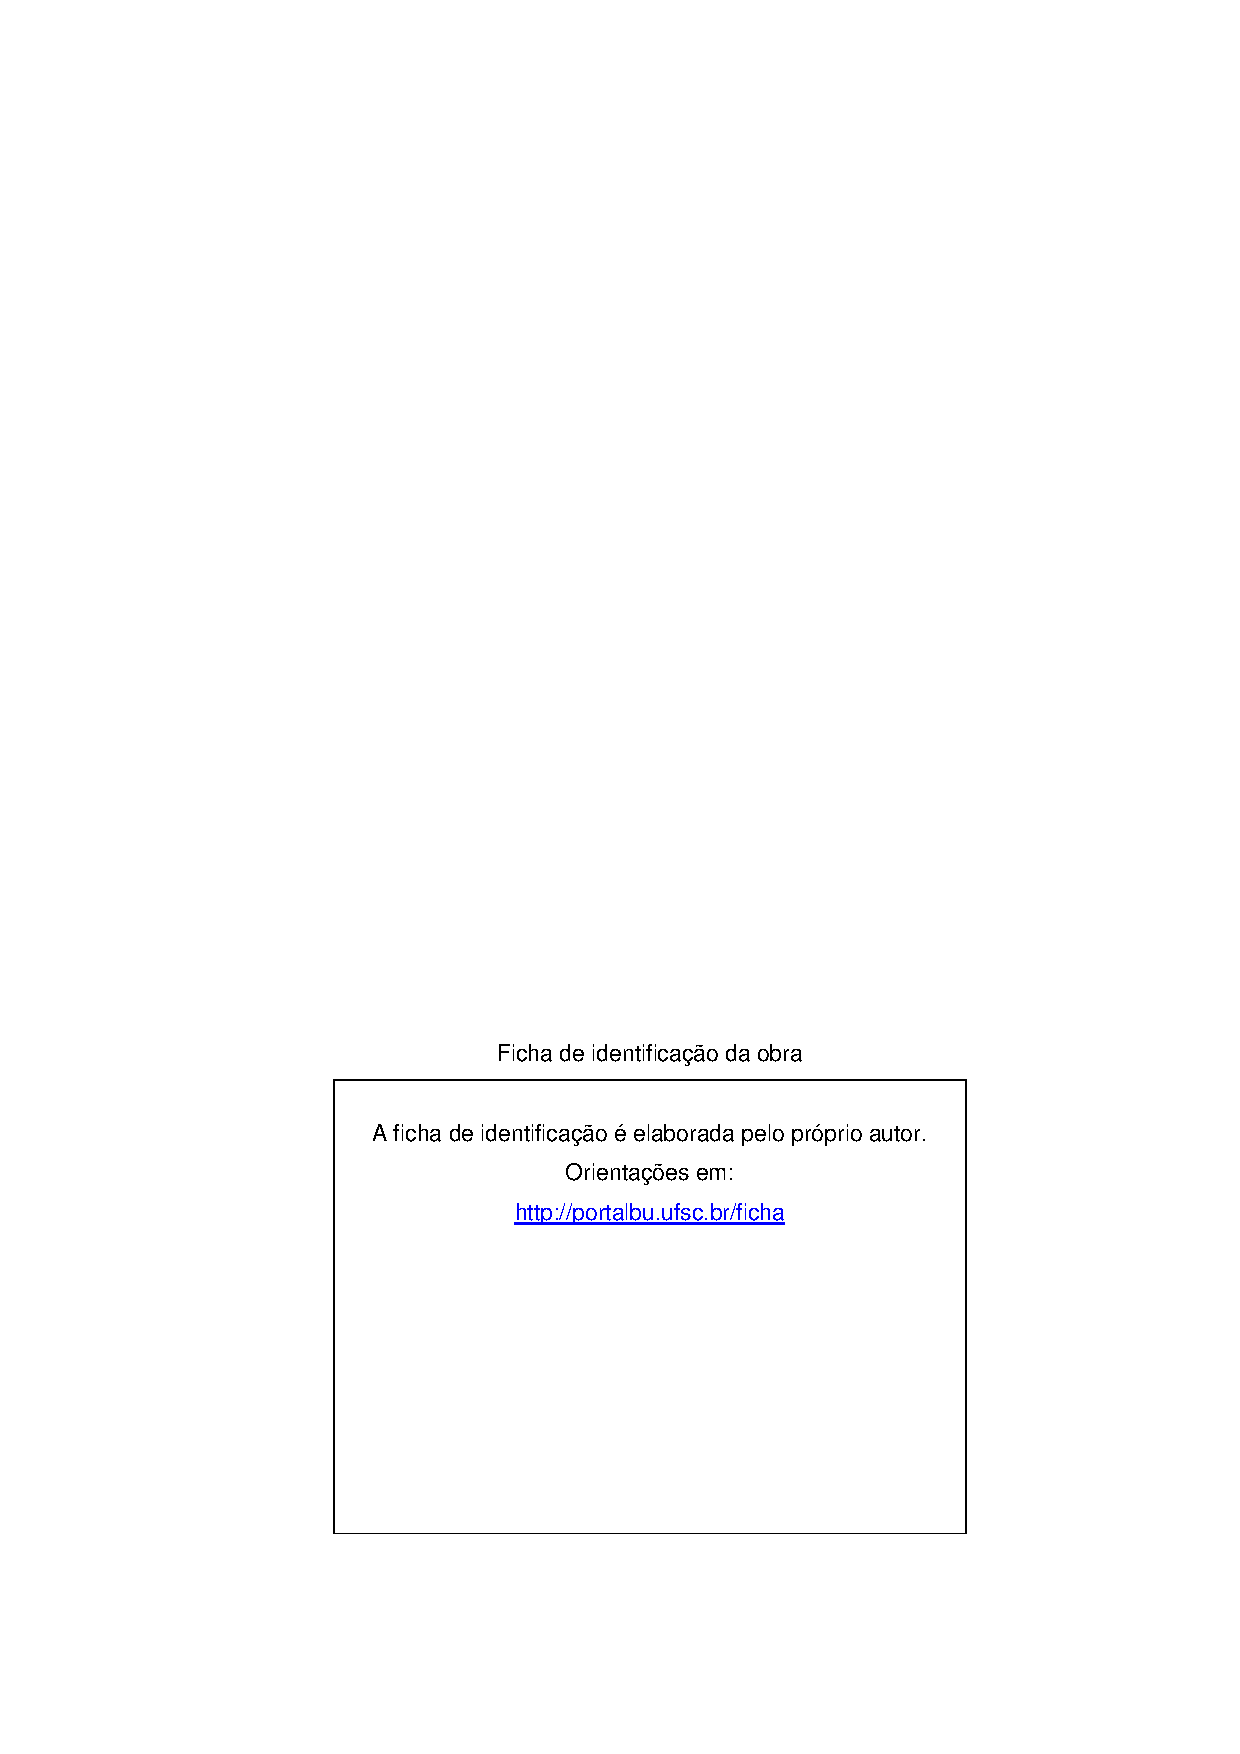
\includepdf{beforetext/Ficha_Catalografica.pdf}
% \end{fichacatalografica}
% ---

% ---
% Inserir folha de aprovação
% ---
\begin{folhadeaprovacao}
	\OnehalfSpacing
	\centering
	\imprimirautor\\%
	\vspace*{10pt}		
	\textbf{\imprimirtitulo}%
	\ifnotempty{\imprimirsubtitulo}{:~\imprimirsubtitulo}\\%
	%		\vspace*{31.5pt}%3\baselineskip
	\vspace*{\baselineskip}
    
	%\begin{minipage}{\textwidth}
	% ~do~\imprimirprograma~do~\imprimircentro~da~\imprimirinstituicao~para~a~obtenção~do~título~de~\imprimirformacao.
	Este~\imprimirtipotrabalho~foi julgado adequado para obtenção do Título de “\imprimirformacao” e aprovado em sua forma final pelo~\imprimirprograma~do~\imprimirinstituicao~--~Campus São Borja. \\
		\vspace*{\baselineskip}
	\imprimirlocal, \imprimirdata. \\
	\vspace*{2\baselineskip}
	% \assinatura{\OnehalfSpacing\imprimircoordenador \\ \imprimircoordenadorRotulo~do Curso}
	\vspace*{2\baselineskip}
	\textbf{Banca Examinadora:} \\
	\vspace*{\baselineskip}
	\assinatura{\OnehalfSpacing\imprimirorientador \\ \imprimirorientadorRotulo}
	%\end{minipage}%
	\vspace*{\baselineskip}
	\assinatura{Prof.(a) xxxx, Dr(a).\\
	Avaliador(a) \\
	Instituição xxxx}

	\vspace*{\baselineskip}
	\assinatura{Prof.(a) xxxx, Dr(a).\\
	Avaliador(a) \\
	Instituição xxxx}


\end{folhadeaprovacao}
% ---

% ---
% Dedicatória
% ---
\begin{dedicatoria}
	\vspace*{\fill}
	\noindent
	% \begin{adjustwidth*}{}{5.5cm}     
    \begin{flushright}
		Este trabalho é dedicado aos meus colegas de \\classe e aos meus queridos pais.
	\end{flushright}
\end{dedicatoria}
% ---

% ---
% Agradecimentos
% ---
\begin{agradecimentos}
	Inserir os agradecimentos aos colaboradores à execução do trabalho. 
	
	Xxxxxxxxxxxxxxxxxxxxxxxxxxxxxxxxxxxxxxxxxxxxxxxxxxxxxxxxxxxxxxxxxxxxxx. 
\end{agradecimentos}
% ---

% ---
% Epígrafe
% ---
\begin{epigrafe}
	\vspace*{\fill}
	\begin{flushright}
		\textit{``Texto da Epígrafe.\\
			Citação relativa ao tema do trabalho.\\
			É opcional. A epígrafe pode também aparecer\\
			na abertura de cada seção ou capítulo.\\
			Deve ser elaborada de acordo com a NBR 10520.''\\
			(Autor da epígrafe, ano)}
	\end{flushright}
\end{epigrafe}
% ---

% ---
% RESUMOS
% ---

% resumo em português
\setlength{\absparsep}{18pt} % ajusta o espaçamento dos parágrafos do resumo
\begin{resumo}
	\SingleSpacing
	O Diabetes Mellitus tipo 2 apresenta elevada proporção de casos não diagnosticados no Brasil, e a triagem na Atenção Primária à Saúde demanda estratégias capazes de priorizar quem encaminhar a exame laboratorial. Diante disso, o presente trabalho teve como objetivo desenvolver um modelo classificatório de aprendizado de máquina para identificar indivíduos com perfil associado à hiperglicemia crônica, definida por hemoglobina glicada igual ou superior a 6,5\%, a partir de variáveis não invasivas da Subamostra Laboratorial da Pesquisa Nacional de Saúde de 2013. A pesquisa, de natureza aplicada e abordagem quantitativa, seguiu a metodologia CRISP-DM sobre uma amostra analítica de 8.451 adultos, dividida em conjuntos de treino e de teste. Foram comparados a Regressão Logística e o \textit{Random Forest}, com aprendizagem sensível ao custo para o tratamento do desbalanceamento das classes, limiar de decisão calibrado para a sensibilidade de 0,80 e explicabilidade por meio do método SHAP. No conjunto de teste, os modelos alcançaram AUC-ROC entre 0,770 e 0,786, e o modelo de referência, o \textit{Random Forest}, obteve sensibilidade de 0,807, encaminhando a exame 40,5\% dos indivíduos, contra 84,0\% de uma regra clínica baseada na idade e no índice de massa corporal. No regime de sensibilidade equiparada à da regra, entretanto, o modelo de referência não cumpriu o critério de sucesso estabelecido, e as probabilidades produzidas mostraram-se descalibradas, de maneira que as saídas foram tratadas como escores de ordenação, e não como estimativas de risco individual. A explicabilidade indicou a idade e a circunferência da cintura como as variáveis de maior contribuição, ordenação que se manteve estável entre dois regimes de cálculo. Conclui-se que o modelo viabiliza uma triagem interpretável, que permite escolher o ponto de operação conforme a capacidade da rede de saúde e fornece a classificação individual acompanhada da contribuição de cada variável, embora a superioridade sobre a regra clínica não tenha sido demonstrada.
	
	\textbf{Palavras-chave}: Diabetes Mellitus tipo 2. Aprendizado de máquina. Triagem. Pesquisa Nacional de Saúde. SHAP.
\end{resumo}

% resumo em inglês
\begin{resumo}[Abstract]
	\SingleSpacing
	\begin{otherlanguage*}{english}
		Type 2 Diabetes Mellitus shows a high proportion of undiagnosed cases in Brazil, and screening in Primary Health Care requires strategies capable of prioritizing who should be referred for laboratory testing. This work aimed to develop a machine learning classification model to identify individuals with a profile associated with chronic hyperglycemia, defined as glycated hemoglobin equal to or greater than 6.5\%, using non-invasive variables from the Laboratory Subsample of the 2013 Brazilian National Health Survey. This applied, quantitative study followed the CRISP-DM methodology on an analytical sample of 8,451 adults, split into training and test sets. Logistic Regression and Random Forest were compared, using cost-sensitive learning to address class imbalance, a decision threshold calibrated for a sensitivity of 0.80, and explainability through the SHAP method. On the test set, the models achieved AUC-ROC between 0.770 and 0.786, and the reference model, the Random Forest, reached a sensitivity of 0.807 while referring 40.5\% of individuals for testing, against 84.0\% for a clinical rule based on age and body mass index. Under the regime of sensitivity matched to that of the rule, however, the reference model did not meet the predefined success criterion, and the estimated probabilities were miscalibrated, so the outputs were treated as ranking scores rather than individual risk estimates. Explainability identified age and waist circumference as the variables with the largest contributions, a ranking that remained stable across two computation regimes. The model enables an interpretable screening that allows the operating point to be chosen according to the capacity of the health network and provides individual classification together with the contribution of each variable, although superiority over the clinical rule was not demonstrated.
		
		\textbf{Keywords}: Type 2 Diabetes Mellitus. Machine learning. Screening. Brazilian National Health Survey. SHAP.
	\end{otherlanguage*}
\end{resumo}

%% resumo em francês 
%\begin{resumo}[Résumé]
% \begin{otherlanguage*}{french}
%    Il s'agit d'un résumé en français.
% 
%   \textbf{Mots-clés}: latex. abntex. publication de textes.
% \end{otherlanguage*}
%\end{resumo}
%
%% resumo em espanhol
%\begin{resumo}[Resumen]
% \begin{otherlanguage*}{spanish}
%   Este es el resumen en español.
%  
%   \textbf{Palabras clave}: latex. abntex. publicación de textos.
% \end{otherlanguage*}
%\end{resumo}
%% ---

{%hidelinks
	\hypersetup{hidelinks}
	% ---
	% inserir lista de ilustrações
	% ---
	\pdfbookmark[0]{\listfigurename}{lof}
	\listoffigures*
	\cleardoublepage
	% ---
	
	% ---
	% inserir lista de quadros
	% ---
	\pdfbookmark[0]{\listofquadrosname}{loq}
	\listofquadros*
	\cleardoublepage
	% ---
	
	% ---
	% inserir lista de tabelas
	% ---
	\pdfbookmark[0]{\listtablename}{lot}
	\listoftables*
	\cleardoublepage
	% ---
	
	% ---
	% inserir lista de abreviaturas e siglas (devem ser declarados no preambulo)
	% ---
	\imprimirlistadesiglas
	% ---
	
	% ---
	% inserir lista de símbolos (devem ser declarados no preambulo)
	% ---
	% \imprimirlistadesimbolos  % desativada: o trabalho não declara símbolos
	% ---
	
	% ---
	% inserir o sumario
	% ---
	\pdfbookmark[0]{\contentsname}{toc}
	\tableofcontents*
	\cleardoublepage
	
}%hidelinks
% ---
% ---

% ----------------------------------------------------------
% ELEMENTOS TEXTUAIS
% ----------------------------------------------------------
\textual

% ---
% 1 - Introdução
% ---
% ----------------------------------------------------------
\chapter{Introdução}
% ----------------------------------------------------------

Segundo \citeonline{da2025uso}, a integração de Tecnologias na Atenção Primária à Saúde (APS) tem promovido avanços significativos na gestão e no cuidado de pacientes crônicos. O uso de abordagens cada vez mais inovadoras é impulsionado pela disponibilidade de dados sociodemográficos e clínicos armazenados em sistemas de informação governamentais. A partir deste cenário, o desenvolvimento de ferramentas que proporcionem suporte à decisão clínica surge como uma solução tecnológica para otimizar a triagem e o direcionamento de recursos públicos, especialmente no combate a doenças crônicas não transmissíveis, cujo impacto estrutural e financeiro sobrecarrega o sistema de saúde \cite{bezerra2025morbidade}.

No contexto da ciência de dados aplicada à saúde, algoritmos de aprendizagem de máquina (\textit{Machine Learning}) destacam-se pela capacidade de identificar padrões sutis e modelar relações não lineares em bases de dados complexas, superando as limitações de escores clínicos tradicionais de pontuação fixa \cite{islam2024comprehensive}. A aplicação de técnicas de mineração de dados sobre pesquisas de abrangência nacional permite o treinamento de modelos classificatórios calibrados especificamente para a realidade fenotípica e social da população brasileira. A possível adoção desse tipo de ferramentas no fluxo assistencial não exige apenas alta precisão, mas também transparência algorítmica, mitigando o efeito "caixa-preta"\footnote{Fenômeno em que um modelo de IA oculta seus processos internos de decisão, tornando o caminho entre a entrada de dados e o resultado final incompreensível para os humanos.} característico de modelos de inteligência artificial \cite{salih2025perspective}.

Alinhado a esta ideia, o presente Trabalho de Conclusão de Curso o propõe o desenvolvimento de um modelo classificatório de \textit{Machine Learning} focado na identificação de indivíduos com perfil de risco metabólico associado ao Diabetes  Mellitus tipo 2 (DM2), operando exclusivamente sobre variáveis não invasivas disponíveis no contexto da APS brasileira visando o apoio à decisão. A fundamentação  teórica, a base de dados utilizada e as decisões metodológicas que orientam o desenvolvimento do modelo são apresentadas nas seções subsequentes deste trabalho.
% ---

% ---
% 2 - Fundamentação Teórica
% ---
% ----------------------------------------------------------
\chapter{Fundamentação Teórica}\label{cap:fundamentacao}
% ----------------------------------------------------------
Este capítulo reúne os conceitos e as diretrizes que fundamentam o desenvolvimento do trabalho, organizados em nove eixos: o Diabetes Mellitus tipo 2 e o desafio na saúde pública; o rastreamento, a APS e as diretrizes clínicas; a Pesquisa Nacional de Saúde de 2013 e os determinantes da saúde; as variáveis antropométricas e clínicas como classificadoras de DM2; a mineração de dados; o pré-processamento e o tratamento de dados; os algoritmos de \textit{Machine Learning}; a avaliação de modelos classificatórios; a Inteligência Artificial Explicável; e a multicolinearidade e seus efeitos sobre a modelagem e a interpretabilidade. Cada eixo dialoga com uma decisão apresentada na Metodologia, de modo que o referencial justifique as etapas do \textit{pipeline} de desenvolvimento do modelo classificatório, em vez de reunir definições isoladas.

\section{O Diabetes Mellitus Tipo 2 e o Desafio na Saúde Pública} \label{sec:dm2-desafio}

O Diabetes Mellitus tipo 2 (DM2) é uma das principais doenças epidêmicas do mundo, representando cerca de 90\% dos casos de diabetes ao redor do globo \cite{who2024diabetes}. Conforme apontado pela literatura especializada em mecanismos patogênicos \cite{mlynarska2025type}, o DM2 é caracterizado por uma progressão silenciosa, na qual a resistência à insulina e o declínio funcional das células beta-pancreáticas\footnote{Células responsáveis pela produção, armazenamento e secreção do hormônio insulina.} antecedem o diagnóstico clínico. Durante anos, ocorre a convivência assintomática com a hiperglicemia\footnote{Condição caracterizada por níveis excessivamente altos de glicose (açúcar) no sangue.}, configurando uma janela temporal propícia a danos celulares progressivos. Essa característica silenciosa colabora para que o diagnóstico clínico ocorra de forma tardia, etapa na qual complicações como nefropatia, retinopatia, neuropatia e doença cardiovascular já podem estar presentes \cite{mlynarska2025type}. 

De acordo com a 11ª edição do Atlas de Diabetes da Federação Internacional de Diabetes \cite{IDF2025}, o Brasil ocupava, em 2024, o 6º lugar no ranking global das dez nações com o maior número de adultos (entre 20 e 79 anos) vivendo com a doença. Além da alta prevalência, o país encontra-se na 9ª posição mundial em volume de pacientes com diabetes não diagnosticado e é classificado como a 3ª nação com o maior gasto total em saúde (em dólares americanos) direcionado ao tratamento da DM. Segundo \textcite{bezerra2025morbidade} o custo médio global de internações de pacientes por Diabetes Mellitus (DM) no Sistema Único de Saúde (SUS), entre janeiro de 2014 e dezembro de 2024, foi de R\$ 832,93, o que evidencia que as consequências geradas pelo DM transcendem a morbidade individual e atingem diretamente a viabilidade financeira do SUS. 

Nesse contexto, conforme as diretrizes atualizadas da Sociedade Brasileira de Diabetes \cite{SBD2025} a triagem precoce configura-se como estratégia de custo-efetividade potencial, ao iniciar o contato com o indivíduo em risco para uma fase anterior ao início de complicações clínicas de alto custo assistencial, já que o diagnóstico precoce e o tratamento nas fases iniciais são fundamentais para a prevenção da evolução para complicações crônicas e a consequente necessidade de encaminhamento para a atenção especializada \cite{Rodacki2025}.

A triagem não se constitui, de forma isolada, como instrumento suficiente para a redução de internações, visto que o desfecho clínico depende de diversos fatores sociais, de acesso à atenção à saúde e do comprometimento individual ao tratamento \cite{geremia2020atenccao}. O que a triagem viabiliza é o encaminhamento assertivo de indivíduos para a confirmação diagnóstica laboratorial, transferindo o foco da intervenção reativa para a prevenção orientada por evidência \cite{brasil2013}. Para fins de parâmetro, o custo unitário do exame de Dosagem de Hemoglobina Glicosilada (HbA1c) tabelado no Sistema de Gerenciamento da Tabela de Procedimentos, Medicamentos e OPM do SUS (SIGTAP) é de R\$ 7,86 \cite{sigtap_hemoglobina_2026}. Embora este valor isoladamente não determine ganhos clínicos ou financeiros, o mesmo ilustra a discrepância de custos entre a fase de rastreamento e a fase de manejo de complicações instaladas \cite{bezerra2025morbidade}, reforçando a relevância econômica do investimento em tecnologias de triagem direcionada na Atenção Primária à Saúde.

\subsection{Rastreamento, APS e Diretrizes Clínicas}\label{sec:rastreamento-aps}
A Sociedade Brasileira de Diabetes publicou, em 2025, uma atualização significativa de suas diretrizes de rastreamento e diagnóstico, cujo marco central é o rebaixamento da idade de início do rastreamento universal de 45 para 35 anos \cite{Rodacki2025}. Essa mudança, baseada em evidências epidemiológicas que apontam para a crescente incidência do DM2 em adultos jovens, representa um avanço substancial na política pública de prevenção, de maneira em que a detecção precoce passa a abranger uma faixa etária anteriormente excluída dos protocolos sistemáticos de triagem \cite{SBD2025}. Adicionalmente, a edição de 2025 incorpora, pela primeira vez, um capítulo dedicado ao uso de ferramentas digitais e Inteligência Artificial no manejo do diabetes, legitimando a adoção de modelos computacionais como suporte à decisão clínica \cite{SBD2025}. Diante disso, o presente trabalho encontra-se diretamente alinhado à direção que a própria sociedade médica de referência nacional aponta como caminho para o aprimoramento do cuidado ao paciente diabético.

Do ponto de vista epidemiológico, a distinção entre triagem populacional e diagnóstico clínico é central para a compreensão dos objetivos e das métricas de desempenho que devem orientar instrumentos de rastreamento \cite{Swaminathan2024, Rodacki2025}. A triagem tem como premissa fundamental a maximização da Sensibilidade (\textit{Recall}), métrica que expressa a capacidade do instrumento de classificar corretamente indivíduos com perfil de risco metabólico associado ao Diabetes Mellitus tipo 2, admitindo-se uma taxa controlada de falsos positivos como custo operacional aceitável, já que o erro de triagem (falso negativo) permite que o paciente permaneça na fase inicial da doença por uma janela de tempo prolongada na qual a hiperglicemia instaura danos celulares crônicos e silenciosos, conforme apontado por \textcite{mlynarska2025type}. O diagnóstico clínico formal exige alta especificidade, priorizando a correta exclusão de indivíduos saudáveis a fim de evitar intervenções terapêuticas desnecessárias \cite{mlynarska2025type, ADA2010, SBD2025}. Conforme apontado por \textcite{Rodacki2025}, o rastreamento torna-se mais eficaz quanto maior a prevalência da doença na população-alvo, de forma com que a seleção de indivíduos com maior probabilidade de resultado positivo visa maximizar a efetividade da iniciativa e a alocação racional dos recursos disponíveis na rede pública de saúde.

No que se refere às ferramentas de triagem atualmente disponíveis para o contexto brasileiro, o \textit{Finnish Diabetes Risk Score} (FINDRISC), adaptado e validado para o português brasileiro por \textcite{conceiccao2020translation}, configura-se como um dos instrumentos mais adotados na Atenção Primária. O escore opera por meio da atribuição de pesos fixos a variáveis como idade, índice de massa corporal, circunferência abdominal, prática de atividade física e histórico familiar de diabetes, gerando uma pontuação ordinal que estratifica o indivíduo em faixas de risco \cite{conceiccao2020translation}. Conforme apontado pela revisão sistemática de \textcite{CarrilloLarco2020} o FINDRISC foi originalmente calibrado em populações europeias, de maneira em que sua aplicação direta a uma população geneticamente heterogênea como a brasileira pode introduzir vieses sistemáticos de classificação. A estrutura de pesos estáticos, embora válida, não permite a captura de interações não lineares entre fatores de risco que, em combinação, elevam expressivamente a probabilidade de hiperglicemia crônica em perfis populacionais específicos, como os documentados nas regiões Norte e Nordeste do Brasil \cite{muzy2021prevalencia}.

O \textit{BrDMrisc}, escore de risco para diabetes incidente derivado da coorte ELSA-Brasil \cite{bracco2026brdmrisc}, representa um avanço metodológico relevante em relação ao FINDRISC ao ser desenvolvido e calibrado sobre dados populacionais brasileiros. Contudo, o instrumento também opera sobre pesos fixos estimados em contexto longitudinal prospectivo, abordagem que, embora metodologicamente robusta, não captura a variabilidade de risco decorrente das interações complexas entre determinantes sociais, antropométricos e clínicos presentes em uma população de heterogeneidade continental como a brasileira \cite{islam2024comprehensive, muzy2021prevalencia}.

A viabilidade de incorporação de modelos classificatórios ao contexto da APS encontra respaldo na capacidade de algoritmos de \textit{Machine Learning} (ML) em capturar padrões complexos em grandes conjuntos de dados, o que inclui interações não lineares entre fatores de risco. Além disso, a crescente digitalização do sistema de saúde brasileiro juntamente da adoção do Prontuário Eletrônico do Cidadão (PEC) no âmbito do Sistema de Informação em Saúde para a Atenção Básica (SISAB) já integra o gerenciamento do cuidado das equipes multidisciplinares \cite{brasil_esus_aps}, configurando uma infraestrutura de captura de dados clínicos rotineiros que, até o presente momento, opera predominantemente como repositório administrativo e não como fonte ativa de inteligência epidemiológica. Contudo, a literatura aponta que o modelo assistencial para condições crônicas ainda opera, de forma predominante, fundamentado na demanda espontânea do paciente \cite{geremia2020atenccao}, de maneira em que indivíduos assintomáticos em fase de risco metabólico elevado permanecem subnotificados até a manifestação clínica de complicações. A aplicação de algoritmos de ML sobre as variáveis rotineiras capturadas pelo PEC apresenta o potencial de romper com essa lógica reativa, transformando o volume de informações clínicas já disponíveis em inteligência epidemiológica ativa, a fim de viabilizar a triagem, classificação e encaminhamento assertivo de indivíduos em fases iniciais para a confirmação diagnóstica laboratorial. A resistência profissional à adoção tecnológica na APS, contudo, figura entre os principais desafios documentados na literatura \cite{geremia2020atenccao}, de forma com que a aceitabilidade clínica de modelos classificatórios depende, em medida expressiva, da capacidade do sistema de apresentar explicações compreensíveis ao profissional de saúde sobre os fatores que motivaram cada classificação. Diante disso, a necessidade de acoplar modelos classificatórios a interfaces de Inteligência Artificial Explicável (XAI) configura-se não apenas como escolha técnica, mas como requisito de adoção clínica \cite{salih2025perspective}.


\section{A Pesquisa Nacional de Saúde (PNS 2013) e os Determinantes da Saúde} \label{sec:pns}

A Pesquisa Nacional de Saúde (PNS) de 2013 é um dos maiores inquéritos populacionais em termos de abrangência e complexidade metodológica já conduzidos no Brasil e integra o Sistema Integrado de Pesquisas Domiciliares (SIPD) do Instituto Brasileiro de Geografia e Estatística \cite{IBGE-SIPD}. O plano amostral adotado pela pesquisa baseia-se na amostragem por conglomerado\footnote{Método probabilístico em que a população é dividida em grupos naturais ou geográficos.} em três estágios de seleção, com estratificação das unidades primárias de amostragem \cite{IBGE_PNS2013_Exames}. No primeiro estágio, foram selecionados os setores censitários ou composições de setores; no segundo estágio, elegeu-se um número fixo de domicílios particulares permanentes em cada unidade primária; e no terceiro estágio, realizou-se a seleção de um único morador adulto por domicílio para a aplicação do questionário individual de saúde. Essa arquitetura amostral complexa acarreta na utilização de pesos amostrais\footnote{Valores numéricos atribuídos a cada indivíduo ou elemento de uma pesquisa que indicam quantas pessoas da população geral aquela observação representa.} nos procedimentos analíticos, a fim de garantir que as estimativas produzidas reflitam a representatividade da população adulta brasileira, e não apenas a distribuição observada na amostra bruta \cite{IBGE_PNS2013_Exames}.

Um diferencial metodológico da edição de 2013 reside na presença de uma Subamostra Laboratorial, na qual foram coletados exames de sangue e urina de 8.952 participantes adultos, incluindo a Dosagem de Hemoglobina Glicosilada (HbA1c) \cite{IBGE_PNS2013_Exames}. A disponibilidade desse marcador laboratorial viabiliza a identificação de indivíduos com hiperglicemia crônica clinicamente significativa independentemente do autorrelato diagnóstico, de modo que o desfecho do presente trabalho (HbA1c $\geq$ 6,5\%, conforme critério da American Diabetes Association \cite{ADA2010}) fundamenta-se em evidência clínica objetiva e não em percepção subjetiva de saúde. A importância dessa distinção é evidenciada pelo fenômeno da subnotificação diagnóstica, já que enquanto a prevalência autorreferida de diabetes na PNS 2013 foi de 6,2\%, a prevalência corrigida por critério laboratorial alcançou 9,4\%, implicando uma proporção nacional de subnotificação de 42,5\%, que atingiu 72,8\% na Região Norte do país \cite{muzy2021prevalencia}. Esse conjunto de evidências demonstra que o autorrelato isolado configura-se como instrumento insuficiente para a vigilância epidemiológica e treinamento de modelos de ML classificatórios para identificação de risco metabólico associado ao DM2, corroborado pela literatura nacional consolidada \cite{iser2015prevalencia, reis2022evolution}.

Em virtude da elevada taxa de não resposta na etapa de coleta biológica, estimada em aproximadamente 52\% em relação à subamostra originalmente prevista, o IBGE desenvolveu e publicou, em 2020, uma Nota Técnica \cite{IBGE} dedicada ao recálculo do peso amostral laboratorial, variável denominada \textit{Peso\_Lab} no arquivo dos microdados disponibilizado pelo IBGE \cite{IBGE_PNS2013_Exames}. Esse peso recalibrado incorpora correções para as distorções provenientes do desenho amostral complexo e das perdas na coleta de material biológico, de forma que as taxas, médias e proporções estimadas a partir da subamostra reflitam o perfil epidemiológico ajustado da população adulta brasileira. Conforme orientação metodológica do IBGE, o Peso\_Lab normalizado para o tamanho da subamostra (n = 8.952) permite a estimação de proporções e taxas representativas, mas não a projeção de volumes populacionais absolutos \cite{IBGE_PNS2013_Exames}.

A diversidade da população brasileira, evidenciada pelas disparidades regionais na prevalência e subnotificação do DM2 documentadas por \textcite{muzy2021prevalencia, iser2015prevalencia, reis2022evolution}, não se explica exclusivamente por fatores biológicos e antropométricos. A literatura especializada em epidemiologia social aponta que variáveis sociodemográficas como escolaridade, raça/cor e macrorregião geográfica atuam como indicadores aproximados dos determinantes sociais da saúde, refletindo iniquidades históricas no acesso à atenção primária, no letramento em saúde e na capacidade de adesão a condutas preventivas \cite{deAlmeida-Pititto09112015}. A escolaridade, em particular, condiciona a capacidade do indivíduo de compreender sinais de alerta, acessar serviços de saúde de forma proativa e aderir a mudanças de estilo de vida recomendadas, de maneira que sua inclusão em modelos classificatórios não visa apenas capturar risco metabólico intrínseco, mas também a dimensão de vulnerabilidade diagnóstica estrutural. A variável raça/cor, por sua vez, captura iniquidades históricas e barreiras de acesso diferencial ao sistema de saúde, além de estresse alostático crônico associado a contextos de discriminação sistêmica, fatores que a literatura epidemiológica brasileira associa a desfechos metabólicos adversos \cite{deAlmeida-Pititto09112015, muzy2021prevalencia}.

Por fim, uma limitação própria ao desenho transversal da PNS 2013 merece fundamentação teórica explícita, visto que ela impõe restrições à inclusão de variáveis comportamentais no modelo classificatório proposto. Em estudos transversais, a exposição e o desfecho são mensurados simultaneamente, impossibilitando estabelecer precedência temporal entre causa e efeito, conforme apontado por \textcite{rothman2008modern}. Diante disso, variáveis comportamentais como prática de exercício físico e padrão alimentar estão sujeitas ao fenômeno de causalidade reversa, na qual o comportamento observado no momento da coleta pode ser consequência do diagnóstico clínico preexistente e não um determinante anterior ao desfecho \cite{rothman2008modern,dimova2020diagnosis}. Como evidenciado por \textcite{dimova2020diagnosis}, o diagnóstico de DM2 frequentemente configura-se como um momento de mudança comportamental induzida pela orientação clínica, na qual o paciente recém-diagnosticado passa a adotar hábitos mais saudáveis por prescrição médica, assim um modelo treinado sobre dados transversais poderia aprender a associar exercício físico e alimentação adequada à presença da doença crônica, invertendo a relação causal real. Diante disso, a exclusão deliberada das variáveis comportamentais do conjunto de classificadores do presente trabalho trata-se de uma decisão metodológica fundamentada na teoria epidemiológica consolidada \cite{rothman2008modern}, a fim de preservar a validade interna das associações aprendidas pelo algoritmo.

\section{Variáveis Antropométricas e Clínicas como Classificadoras de DM2}\label{sec:variaveis}

A seleção das variáveis classificadoras voltadas à identificação de risco metabólico associado ao DM2 fundamentou-se em evidências clínicas e epidemiológicas consolidadas, de modo que cada variável incorporada ao conjunto de classificadores apresente justificativa biológica e empírica para a sua associação com o desfecho de hiperglicemia crônica. Neste trabalho, as variáveis antropométricas constituem o núcleo do bloco biológico do modelo e, de acordo com \textcite{mlynarska2025type}, foram selecionadas em razão de sua capacidade de capturar dimensões complementares do fenótipo individual, em especial aquelas associadas à adiposidade visceral\footnote{Acúmulo de gordura intra-abdominal ao redor de órgãos vitais como fígado, pâncreas e intestinos.} e à resistência à insulina\footnote{Condição em que o corpo não responde adequadamente à insulina, hormônio que facilita a entrada de glicose nas células.}.

O Índice de Massa Corporal (IMC), calculado pela razão entre o peso corporal em quilogramas e o quadrado da altura em metros, fórmula clássica de Quetelet \cite{eknoyan2008adolphe}, constitui o preditor basal de sobrepeso e obesidade mais amplamente utilizado em estudos epidemiológicos e diretrizes clínicas, em virtude de sua simplicidade e da disponibilidade de pontos de corte internacionalmente consolidados \cite{mlynarska2025type}. Entretanto, a literatura de \textcite{Feller2010} evidencia que o IMC apresenta limitações relevantes para a avaliação do risco metabólico, visto que a medida não distingue adiposidade visceral de adiposidade subcutânea\footnote{Camada de gordura localizada logo abaixo da pele.}, compartimentos adiposos com propriedades metabólicas substancialmente distintas \cite{Feller2010}. Os textos de \textcite{Feller2010,mlynarska2025type} relatam que o tecido adiposo visceral, ao contrário do subcutâneo, é metabolicamente ativo e secreta adipocinas inflamatórias que induzem resistência à insulina e disfunção endotelial\footnote{Alteração precoce na camada que reveste o interior dos vasos sanguíneos (endotélio).}, configurando-se como determinante patogênico do DM2.

Diante dessa limitação, a Circunferência da Cintura (CC) emerge como preditor superior para a quantificação da adiposidade visceral. O estudo de \textcite{Feller2010}, conduzido com 9.753 homens e 15.491 mulheres participantes da coorte EPIC-Potsdam\footnote{Projeto populacional de coorte prospectiva na Alemanha.}, demonstrou que um incremento de 1 cm na circunferência da cintura está associado a um aumento de 8\% no risco relativo de desenvolvimento de DM2, tanto em homens quanto em mulheres \cite{Feller2010}. De forma ainda mais expressiva, o estudo evidenciou que indivíduos com IMC inferior a 25 kg/m² mas com circunferência da cintura elevada apresentaram risco relativo de DM2 de 3,62 vezes em homens e 2,74 vezes em mulheres em comparação ao grupo de referência, risco equivalente ou superior ao observado em indivíduos com pré-obesidade e cintura normal \cite{Feller2010}. Esse achado evidencia que a utilização isolada do IMC como critério de triagem configura-se insuficiente para a identificação de perfis de risco metabólico relevantes na população adulta, de modo que a mensuração complementar da circunferência da cintura se faz relevante para uma classificação mais precisa e clinicamente correta. Na Subamostra Laboratorial da PNS 2013, a aferição da circunferência da cintura seguiu o protocolo padronizado pelo IBGE, com medição realizada no ponto médio entre a borda inferior da última costela e a borda superior da crista ilíaca, em conformidade com a recomendação metodológica da Organização Mundial da Saúde \cite{IBGE_PNS2013_Exames}.

O estudo longitudinal de \textcite{Son2016} evidencia que a razão Cintura-Estatura (RCEst), derivada da divisão entre a circunferência da cintura e a altura do indivíduo, deve ser incluída como variável auxiliar a fim de capturar a adiposidade visceral ajustada pela estatura individual, já que essa dimensão não é abrangida de forma integral pelo IMC ou pela circunferência da cintura em valor absoluto isoladamente. O estudo demonstra que a RCEst apresenta a vantagem de contextualizar o depósito de gordura central em relação ao porte corporal do indivíduo, de forma que dois indivíduos com a mesma circunferência absoluta possam apresentar perfis de risco visceral distintos em função da estatura. A partir dessa fundamentação, o bloco antropométrico candidato reúne três aspectos complementares do fenótipo corporal: a magnitude geral do acúmulo adiposo (IMC), a concentração de gordura na região abdominal (CC) e a adiposidade visceral ajustada pela estrutura corporal (RCEst) \cite{mlynarska2025type, Feller2010,Son2016}. A permanência de cada uma dessas variáveis no modelo final ficou condicionada ao diagnóstico de multicolinearidade descrito na Metodologia.

Segundo a \textcite{SBD2019}, a Hipertensão Arterial Sistêmica (HAS), em conjunto com a dislipidemia\footnote{Nome dado aos níveis alterados (geralmente altos) de gorduras, como colesterol e triglicerídeos, no sangue.} e a adiposidade central, forma o ``tripé'' clássico da Síndrome Metabólica, condição clínica de alta prevalência na população brasileira e fortemente associada à resistência à insulina e ao desenvolvimento do DM2. No presente trabalho, a pressão arterial foi considerada em duas dimensões complementares: a medida objetiva (pressões sistólica e diastólica aferidas durante a coleta da PNS 2013) e o autorrelato diagnóstico de HAS. Optou-se por considerar as duas fontes em razão da premissa central do trabalho, a qual prioriza dados objetivos sobre o autorrelato em razão do fenômeno documentado de subnotificação diagnóstica na população brasileira por \textcite{muzy2021prevalencia}, ao mesmo tempo em que preserva a dimensão de consciência diagnóstica do indivíduo como proxy\footnote{Variáveis utilizadas como indicadores indiretos de um conceito que não pode ser mensurado diretamente.} de acesso ao sistema de saúde.

A dislipidemia, operacionalizada por meio do diagnóstico autorreferido de colesterol alto (variável Q060 da PNS 2013), é incorporada ao modelo em razão do seu papel consolidado na fisiopatologia da Síndrome Metabólica \cite{mlynarska2025type, SBD2019}. Adicionalmente, a partir da combinação de HAS combinada, dislipidemia autorreferida e presença de obesidade (definida por IMC $\geq$ 30 kg/m² ou CC $\geq$ 80 cm em mulheres ou $\geq$ 94 cm em homens \cite{SBD2019}), foi desenvolvida a variável derivada \textit{Multimorbidade Metabólica}, operacionalizada como escore ordinal de zero a três, a fim de viabilizar a captura de interações sinérgicas entre condições clínicas que, isoladamente, poderiam não atingir o limiar de risco identificável pelo algoritmo, mas que em combinação elevam expressivamente a probabilidade de hiperglicemia crônica clinicamente significativa \cite{SBD2019, rzewuska2017epidemiology}.

Por fim, o estado de saúde autoavaliado (variável N001 da PNS 2013), internacionalmente referido como \textit{Self-Rated Health} (SRH), foi incorporado ao conjunto de classificadores em virtude da sua consolidação, em estudos epidemiológicos transversais e longitudinais, como preditor de desfechos crônicos e de mortalidade em populações adultas \cite{Rantanen2019}. No contexto específico da identificação de DM2 não diagnosticado, o estudo de \textcite{Rantanen2019} demonstra que a SRH apresenta uma alta relevância, já que, segundo os autores, indivíduos com hiperglicemia crônica não diagnosticada frequentemente manifestam sintomas genéricos em estágios pré-clínicos, a exemplo de fadiga, sede anormal leve e poliúria\footnote{Termo médico utilizado para descrever a produção e eliminação de quantidades excessivas de urina.}, capaz de impactar a percepção subjetiva de saúde antes mesmo da formalização diagnóstica.

\section{Mineração de Dados} \label{sec:mineracao}

De acordo com \textcite{mining2006introduction}, a mineração de dados (\textit{Data Mining}) configura-se como um conjunto de ferramentas e algoritmos que permitem a análise e solução de problemas que demandariam esforço manual massivo ou simplesmente ficariam sem solução. A mesma também pode ser definida como um conjunto de ferramentas ou técnicas que possibilitam identificar relações, padrões e regularidades que não seriam detectáveis por análise humana direta. No contexto do presente trabalho, a aplicação dessas técnicas sobre bases de dados populacionais, como os microdados da PNS 2013, viabiliza a transformação de informações clínicas e sociodemográficas coletadas em inteligência epidemiológica ativa, de maneira que possíveis padrões presentes na população possam ser identificados de forma sistemática \cite{islam2024comprehensive}.

A fim de orientar projetos de mineração de dados de forma estruturada e reprodutível, o modelo \textit{Cross Industry Standard Process for Data Mining} (CRISP-DM) foi desenvolvido em 1996 por uma parceria de empresas europeias liderada por Daimler-Benz, SPSS (\textit{Statistical Package for the Social Sciences}), NCR (\textit{National Cash Register}) e Ohra, sendo formalizado e publicado por Wirth e Hipp em 2000 \cite{wirth2000crisp}. O CRISP-DM organiza o ciclo de vida de um projeto de mineração de dados em seis fases iterativas: Compreensão do Negócio (\textit{Business Understanding}), Compreensão dos Dados (\textit{Data Understanding}), Preparação dos Dados (\textit{Data Preparation}), Modelagem (\textit{Modeling}), Avaliação (\textit{Evaluation}) e Implantação (\textit{Deployment}) \cite{wirth2000crisp}. A natureza iterativa do modelo é um dos seus diferenciais fundamentais, já que as fases não são executadas de forma linear e sequencial, e sim de maneira cíclica, de modo que ações e descobertas realizadas em fases avançadas do processo possam justificar retornos a etapas anteriores a fim de refinar os dados, as hipóteses ou as decisões de modelagem \cite{wirth2000crisp}. Diante disso, o CRISP-DM favorece a rastreabilidade metodológica desde a concepção inicial do problema até a validação da solução, característica relevante para a reprodutibilidade científica de projetos baseados em dados públicos.

A predominância do CRISP-DM como \textit{framework} para projetos de ciência de dados e mineração de dados é amplamente corroborada pela literatura especializada. Conforme evidenciado pela revisão sistemática conduzida por \textcite{schroer2021systematic}, o CRISP-DM consolida-se como o modelo mais adotado em projetos de \textit{Machine Learning} e mineração de dados ao redor do mundo, em virtude de sua flexibilidade para adaptação a diferentes domínios de aplicação e da clareza com que organiza as responsabilidades e entregas de cada fase do projeto. Embora a revisão aponte que o modelo original pode necessitar de adaptações de \textit{Design Thinking} para atender a requisitos modernos de interação com o usuário final, a robustez do CRISP-DM para o tratamento de dados estruturados consolida o mesmo como uma base ideal para o processamento de microdados populacionais como os que estão presentes na Subamostra Laboratorial da PNS 2013 \cite{schroer2021systematic}.

Conforme documentado por \textcite{shimaoka2024evolution}, o modelo original do CRISP-DM foi objeto de revisões e extensões metodológicas que buscaram alinhar suas fases ao ciclo de desenvolvimento de sistemas de inteligência artificial, incorporando práticas contemporâneas de engenharia de dados, gestão de experimentos e monitoramento de modelos em produção. Diante disso, essa metodologia permanece como referência central para projetos que, como o presente trabalho, combinam processamento de dados com desenvolvimento de modelos classificatórios e implantação de protótipos funcionais \cite{shimaoka2024evolution}.

\section{Pré-processamento e Tratamento de Dados} \label{sec:pre-processamento}

\textcite{hastie2009elements} abordam extensivamente como a qualidade dos dados submetidos ao treinamento de um modelo classificatório constitui um dos determinantes mais críticos de seu desempenho. Em bases de dados baseadas em inquéritos populacionais como a Subamostra Laboratorial da PNS 2013, é comum a presença de valores ausentes, decorrentes de não respostas, erros de coleta ou do desenho condicional do questionário, ponto abordado diretamente na nota técnica disponibilizada sobre a amostra \cite{IBGE}. Soma-se a isso o desbalanceamento entre as classes do desfecho, situação na qual a classe de interesse representa proporção significativamente menor que a classe majoritária \cite{pertiwi2020comparison}. Por esta razão, a etapa de pré-processamento dos dados se faz necessária para garantir a integridade estatística do conjunto de treino e a validade das associações aprendidas pelo algoritmo ao longo do processo de modelagem.

Além disso, a presença de valores ausentes é um dos desafios mais comuns no tratamento de dados \cite{hastie2009elements}. Dentre as abordagens disponíveis, a substituição por medidas de tendência central, como a substituição pela média ou pela mediana da variável, é uma alternativa de simples implementação, contudo apresenta uma limitação, já que ao desconsiderar as relações multivariadas entre os preditores, pode introduzir distorções na distribuição dos dados, produzindo registros implausíveis, onde a combinação de valores não corresponde a nenhum perfil real da população estudada \cite{hastie2009elements}. Já a imputação por meio do algoritmo \textit{K-Nearest Neighbors} (KNN) opera sobre a estrutura de similaridade multivariada dos dados, ou seja, cada valor ausente é preenchido com base na média ponderada dos $k$ vizinhos mais próximos no espaço multidimensional das demais variáveis disponíveis \cite{pedregosa2011scikit, pertiwi2020comparison}. Por meio desta abordagem, os valores substituídos preservam a estrutura de correlação entre si, de forma com que os registros resultantes sejam coerentes com os padrões observados na base de dados.

Em relação ao tratamento do desbalanceamento de classes, a literatura discute diversas técnicas. No contexto do presente trabalho, concentrou-se em dois tipos de métodos, a reamostragem no nível dos dados (\textit{data-level}), como o SMOTE (\textit{Synthetic Minority Over-sampling Technique}), e no nível algorítmico (\textit{algorithm-level}), como a aprendizagem sensível ao custo (\textit{Cost-Sensitive Learning}) \cite{araf2024costsensitive}. Conforme evidenciado pela revisão sistemática conduzida por \textcite{araf2024costsensitive}, as abordagens de reamostragem que geram instâncias sintéticas, como o SMOTE, apresentam limitações em contextos onde os dados originais são resultantes de desenhos amostrais complexos, visto que a criação de observações artificiais quebra a estrutura de ponderação amostral utilizada para representatividade populacional das estimativas \cite{10.1371/journal.pone.0280387}. 

Já a aprendizagem sensível ao custo opera diretamente sobre a função de perda do algoritmo, atribuindo penalizações aos erros de classificação de cada classe, fazendo com que o custo de classificar incorretamente um indivíduo da classe minoritária seja proporcionalmente superior ao custo de um erro na classe majoritária, sem a necessidade de alterar a distribuição original dos dados de treino \cite{araf2024costsensitive}. No contexto da biblioteca \textit{scikit-learn} \cite{pedregosa2011scikit}, essa estratégia é realizada por meio do hiperparâmetro \texttt{class\_weight='balanced'}, cuja função é atribuir pesos inversamente proporcionais à frequência de cada classe no conjunto de treino, ou seja, o algoritmo é induzido a tratar os erros de classificação da classe minoritária com maior peso durante a otimização \cite{pedregosa2011scikit}. Essa característica torna a aprendizagem sensível ao custo adequada a este trabalho, pois a preservação da estrutura amostral original viabiliza a manutenção dos pesos laboratoriais (\textit{Peso\_Lab}) recalculados pelo IBGE \cite{ibge2013pns}, de forma com que a representatividade populacional das estimativas produzidas na fase de Análise Exploratória de Dados não seja comprometida pelo tratamento do desbalanceamento na fase de modelagem.


\section{Algoritmos de \textit{Machine Learning}} \label{sec:algoritmos-ml}

A seleção dos algoritmos de classificação supervisionada constitui uma das decisões de maior impacto em projetos de \textit{Machine Learning}. No presente trabalho, foram selecionados dois algoritmos: a Regressão Logística, utilizada como modelo de linha de base (\textit{baseline}) interpretável, e o \textit{Random Forest}, escolhido como modelo de maior capacidade representacional para a captura de interações não lineares entre as variáveis classificadoras.

A Regressão Logística constitui um modelo estatístico clássico e linear cuja função é estimar a probabilidade de ocorrência de um desfecho binário a partir de um conjunto de variáveis explicativas \cite{hastie2009elements}. O modelo opera por meio da função logística, que transforma a combinação linear dos preditores em uma probabilidade restrita ao intervalo entre zero e um, viabilizando a classificação binária de indivíduos em relação ao desfecho de interesse \cite{hastie2009elements}. Conforme evidenciado por \textcite{nusinovici2020logistic}, a Regressão Logística apresenta desempenho comparável ao de algoritmos de \textit{Machine Learning} mais complexos em tarefas de classificação de doenças crônicas, de forma com que sua adoção como \textit{baseline}\footnote{Modelo inicial simples usado como ponto de partida para comparar e justificar o desempenho de algoritmos mais complexos.} se justifica tanto pela transparência paramétrica quanto pela consolidação histórica em estudos epidemiológicos. A interpretabilidade do modelo reside na possibilidade de extrair, a partir dos coeficientes estimados, a razão de chances (\textit{odds ratio}) associada a cada variável, métrica amplamente utilizada em epidemiologia clínica para quantificar a magnitude da associação entre um preditor e o desfecho \cite{nusinovici2020logistic}.

O \textit{Random Forest} constitui um algoritmo de aprendizagem por conjunto (\textit{ensemble}) que combina as classificações de múltiplas árvores de decisão independentes a fim de produzir uma classificação final mais robusta e generalizada do que qualquer árvore individual seria capaz de fornecer \cite{islam2024comprehensive}. Cada árvore é treinada sobre uma subamostra aleatória do conjunto de treino, e em cada nó de divisão apenas um subconjunto aleatório de variáveis é avaliado como candidato, de maneira em que as árvores individuais tornam-se descorrelacionadas entre si e a agregação das saídas das árvores produz classificações de menor variância \cite{islam2024comprehensive}. A principal vantagem do \textit{Random Forest} em relação à Regressão Logística, no contexto do presente trabalho, reside na sua capacidade de capturar interações não lineares entre os classificadores, a exemplo da interação entre idade avançada, circunferência da cintura elevada e baixa escolaridade em regiões de menor acesso à atenção primária, padrões que um modelo linear não conseguiria representar de forma adequada \cite{islam2024comprehensive}. Adicionalmente, a compatibilidade do \textit{Random Forest} com o método \textit{TreeExplainer} da biblioteca SHAP viabiliza a decomposição das contribuições individuais de cada variável para cada classificação realizada pelo modelo, requisito para a interpretabilidade clínica das saídas do protótipo \cite{salih2025perspective}.

\section{Avaliação de Modelos Classificatórios} \label{sec:avaliacao}

A avaliação do desempenho de modelos classificatórios constitui a etapa central no desenvolvimento de sistemas de \textit{Machine Learning} aplicados à saúde, visto que a escolha das métricas deve estar alinhada aos objetivos clínicos do instrumento e às consequências assimétricas dos diferentes tipos de erro classificatório \cite{Swaminathan2024}. Nesse sentido, a Matriz de Confusão é o instrumento central de avaliação em tarefas de classificação binária, organizando os quatro possíveis resultados de uma classificação: Verdadeiros Positivos (VP), Verdadeiros Negativos (VN), Falsos Positivos (FP) e Falsos Negativos (FN) \cite{Swaminathan2024}. A partir dessa estrutura, resultam as métricas utilizadas no presente trabalho.

A Sensibilidade (\textit{Recall}) expressa a capacidade do modelo de identificar corretamente os indivíduos portadores da condição, configurando-se como a métrica prioritária em instrumentos de triagem populacional:

\begin{equation}
\text{Sensibilidade} = \frac{VP}{VP + FN} \quad \text{ \cite{Swaminathan2024}}
\end{equation}

\noindent A Especificidade quantifica a capacidade do modelo de identificar corretamente os indivíduos saudáveis, de modo que valores altos implicam baixa taxa de encaminhamentos desnecessários:

\begin{equation}\text{Especificidade} = \frac{VN}{VN + FP} \text{ \cite{Swaminathan2024}}
\end{equation}

\noindent O \textit{F1-Score} constitui a média harmônica entre Precisão e Sensibilidade, cuja função é equilibrar ambas as métricas em cenários de desbalanceamento de classes \cite{Swaminathan2024}:

\begin{equation}F1 = 2 \times \frac{\text{Precisão} \times \text{Sensibilidade}}{\text{Precisão} + \text{Sensibilidade}} \text{ \cite{Swaminathan2024}}
\end{equation}

\noindent A Área Sob a Curva ROC (AUC-ROC) avalia a capacidade discriminativa global do modelo ao plotar a Sensibilidade em função da taxa de Falsos Positivos ao longo de todos os limiares de classificação possíveis. Valores próximos a 1 indicam elevada capacidade discriminativa, enquanto 0,5 equivale à classificação aleatória \cite{fawcett2006introduction, powers2020evaluation}.

A Validação Cruzada Estratificada com $k = 5$ \textit{folds} divide o conjunto de treino em $k$ partições, utilizando, em cada iteração, $k-1$ partições para treinamento e uma para validação \cite{pedregosa2011scikit}. A estratificação garante que a proporção da classe positiva seja preservada em cada partição, característica relevante em cenários de desbalanceamento \cite{pertiwi2020comparison}. A média e o desvio padrão das métricas ao longo das $k$ iterações descrevem a variação do desempenho entre partições.


\section{Inteligência Artificial Explicável (XAI)} \label{sec:xai}

A crescente adoção de algoritmos de aprendizagem de máquina em diversos contextos trouxe consigo um desafio: algoritmos de alta capacidade, como o \textit{Random Forest}, operam por meio de estruturas computacionais de alta complexidade, nas quais a classificação final resulta da agregação de centenas ou milhares de árvores de decisão individuais, de maneira em que a contribuição de cada variável para o resultado final torna-se vaga e praticamente impossível de interpretar por meio de análise direta \cite{salih2025perspective}. Esse fenômeno, amplamente referido na literatura como o dilema da ``caixa-preta'' (\textit{black box}), caracteriza-se como barreira à adoção de modelos de \textit{Machine Learning} em ambientes clínicos, visto que profissionais de saúde e gestores do sistema público necessitam compreender os fundamentos das classificações produzidas a fim de assumir a responsabilidade ética pelas condutas assistenciais delas derivadas \cite{salih2025perspective}.

No contexto da Atenção Primária à Saúde brasileira, essa barreira apresenta dimensões adicionais. A literatura evidencia que a resistência profissional à adoção de tecnologias digitais está entre os principais desafios à continuidade do modelo assistencial na APS \cite{geremia2020atenccao}, e a aceitabilidade de um sistema classificatório por parte das equipes multidisciplinares depende da capacidade do sistema de justificar suas saídas em linguagem compreensível ao usuário. Diante disso, a integração de técnicas de Inteligência Artificial Explicável (XAI) ao modelo proposto no presente trabalho não é apenas uma escolha técnica, mas um requisito de viabilidade do protótipo desenvolvido \cite{geremia2020atenccao, salih2025perspective}.

A Inteligência Artificial Explicável (XAI) é caracterizada como um conjunto de métodos, técnicas e ferramentas cuja função é transformar modelos de aprendizagem de máquina em sistemas onde as decisões sejam compreensíveis e auditáveis por usuários humanos, sejam eles especialistas técnicos ou profissionais de domínio \cite{salih2025perspective}. Dentre os métodos de XAI disponíveis na literatura, o SHAP (\textit{SHapley Additive exPlanations}) se sobressai como a abordagem de maior rigor matemático e mais ampla adoção em aplicações clínicas \cite{salih2025perspective}. O SHAP fundamenta-se na teoria dos jogos cooperativos, mais especificamente no conceito de valores de Shapley, desenvolvido por Lloyd Shapley em 1953, que define a contribuição de cada participante em um jogo cooperativo com base na sua contribuição marginal média em todas as coalizões possíveis de participantes \cite{salih2025perspective}. Trazendo este conceito para o contexto da explicabilidade de modelos de \textit{Machine Learning}, essa teoria permite que cada variável classificatória seja tratada como um ``jogador'' e que a classificação final do modelo seja decomposta na contribuição individual de cada variável.

A análise via SHAP abrange duas dimensões de interpretabilidade. A dimensão global, calculada sobre o conjunto de teste completo, produz uma visão agregada da importância relativa de cada variável nas classificações do modelo e permite confrontar as associações aprendidas pelo algoritmo com a evidência epidemiológica consolidada \cite{salih2025perspective}. A dimensão local decompõe a contribuição de cada variável no escore atribuído a um indivíduo, de modo que cada classificação venha acompanhada da justificativa do algoritmo \cite{salih2025perspective}. Os valores de Shapley expressam contribuições estatísticas observadas em dados transversais e não constituem relações causais nem predições de desenvolvimento futuro da condição clínica avaliada.

\section{Multicolinearidade e seus Efeitos sobre a Modelagem e a Interpretabilidade}\label{sec:multicolinearidade}

Segundo \textcite{Salih2024} a multicolinearidade é definida como um fenômeno no qual múltiplas características em modelos de aprendizado de máquina são altamente correlacionadas entre si. Conforme abordado por \textcite{Senaviratna2019}, no contexto da Regressão Logística, a multicolinearidade infla a variância dos coeficientes estimados, tornando as estimativas instáveis e comprometendo a confiabilidade dos testes de significância individual. No que se refere aos modelos baseados em árvores de decisão, como o \textit{Random Forest}, a multicolinearidade apresenta impacto reduzido sobre o desempenho classificatório, visto que esses algoritmos selecionam variáveis de forma iterativa com base em critério de ganho de informação, sendo naturalmente mais robustos à presença de correlações entre preditores \cite{Chan2022}.

Entretanto, \textcite{Salih2024} evidencia que a robustez classificatória dos modelos de árvore não se estende ao plano da interpretabilidade via SHAP, visto que, na versão original, o método assume independência estatística entre variáveis para a geração das explicações. Quando duas variáveis possuem forte correlação entre si e se correlacionam com o desfecho, apenas uma delas tende a receber um valor SHAP elevado, já que a inclusão da segunda variável no modelo não acrescenta ganho informacional significativo em relação à primeira. Assim, o valor SHAP resultante não captura o impacto real de cada variável sobre o desfecho quando as \textit{features} são colineares. Dessa forma, a lista de variáveis mais relevantes produzida pelo método pode se tornar incompleta ou enviesada em favor de uma das variáveis do par correlacionado \cite{Salih2024}. Esse fenômeno é particularmente relevante para o presente trabalho, visto que algumas das variáveis selecionadas, apresentadas na Metodologia, são clinicamente complementares, porém estatisticamente correlacionadas entre si. 

A revisão conduzida por \textcite{Salih2024} identificou sete abordagens propostas na literatura para mitigar o impacto da multicolinearidade sobre os métodos de XAI, dentre as quais se destacam o \textit{Modified Index Position} (MIP), o \textit{Extended Kernel SHAP} e o \textit{Multi-Collinearity Corrected} (MCC). Entretanto, o autor constata que nenhum método de XAI disponível mitiga, por natureza, o impacto da multicolinearidade sobre suas explicações, de forma com que o tratamento desse fenômeno demanda intervenções metodológicas complementares por parte do pesquisador \cite{Salih2024}.


% ---

% ---
% 3 - Metodologia
% ---
% ----------------------------------------------------------
\chapter{Metodologia}\label{cap:metodologia}
% ----------------------------------------------------------

\section{Caracterização da Pesquisa}\label{sec:caracterizacao}

O presente trabalho caracteriza-se como uma pesquisa de natureza aplicada e abordagem quantitativa \cite{prodanov2013metodologia}, conduzida sobre dados secundários provenientes de um inquérito populacional de desenho transversal, no qual a exposição e o desfecho são mensurados simultaneamente \cite{rothman2008modern}. Para a condução das etapas do projeto, foi adotado o modelo \textit{Cross Industry Standard Process for Data Mining} (CRISP-DM), que, conforme evidenciado pela revisão sistemática conduzida por \textcite{schroer2021systematic}, consolida-se como o modelo de processo mais utilizado para orientar projetos de ciência de dados, mineração de dados e \textit{Machine Learning}. Em virtude de sua natureza iterativa, o modelo favorece a rastreabilidade desde a concepção do problema até a validação da solução, motivo pelo qual foi escolhido como \textit{framework} deste trabalho.

Embora a literatura aponte que o modelo original pode necessitar de adaptações de \textit{Design Thinking}\footnote{Abordagem centrada no ser humano para resolver problemas complexos e promover a inovação.} para atender a requisitos modernos de interação com o usuário final \cite{schroer2021systematic}, a robustez do CRISP-DM para o tratamento de dados estruturados torna-o adequado ao processamento dos microdados da Pesquisa Nacional de Saúde (PNS). A fim de suprir a lacuna de usabilidade apontada, a Inteligência Artificial Explicável (XAI) foi integrada ao processo por meio do método SHAP \cite{salih2025perspective}, visando proporcionar a transparência necessária à aceitabilidade do modelo no contexto da APS brasileira. Além disso, cada decisão tomada ao longo da execução e não prevista no projeto de pesquisa foi registrada juntamente com o motivo que a originou e com a sua relação com o projeto, de maneira que o percurso metodológico pudesse ser auditado, conforme descrito no capítulo de Desenvolvimento.

\section{Considerações Éticas}

Para o desenvolvimento deste trabalho, foram utilizados exclusivamente microdados públicos e anonimizados, disponibilizados pelo Instituto Brasileiro de Geografia e Estatística (IBGE) por meio da Subamostra Laboratorial da Pesquisa Nacional de Saúde de 2013 \cite{IBGE_PNS2013_Exames}. A Resolução CNS nº 466/2012 estabelece as diretrizes gerais para as pesquisas envolvendo seres humanos, definindo-as de forma a incluir o manejo de seus dados, e remete a uma resolução complementar as especificidades das pesquisas que se utilizam de metodologias próprias das ciências humanas e sociais \cite{brasil2012resolucao466}, papel exercido pela Resolução CNS nº 510/2016. Diante disso, em virtude da natureza secundária dos dados e da impossibilidade de identificação individual dos participantes, a pesquisa dispensou a submissão e a aprovação por Comitê de Ética em Pesquisa (CEP), conforme o artigo 1º, parágrafo único, incisos II e III, da Resolução CNS nº 510/2016, que excluem do registro e da avaliação pelo sistema CEP/CONEP as pesquisas que utilizam informações de acesso público e de domínio público \cite{cns2016resolucao510}. A íntegra das duas resoluções é apresentada nos Anexos~\ref{anexo:res510} e~\ref{anexo:res466}.

\section{Base de Dados e Amostra Analítica}\label{sec:base-dados}

A escolha da Pesquisa Nacional de Saúde (PNS) de 2013, em detrimento da edição de 2019, deu-se em virtude de uma diferença metodológica decisiva entre as duas pesquisas, visto que somente a edição de 2013 contou com a Subamostra Laboratorial, na qual foram coletados exames de Hemoglobina Glicada (HbA1c)\footnote{Exame de sangue que mede a média dos níveis de glicose no sangue nos últimos dois a três meses, essencial para o diagnóstico e controle do diabetes.} de 8.952 participantes adultos \cite{IBGE_PNS2013_Exames}. Por meio desta variável laboratorial, o presente trabalho viabilizou um desfecho clínico objetivo (HbA1c $\geq$ 6,5\%) como referência para o modelo, em substituição ao diagnóstico autorreferido, abordagem reconhecida pela literatura como suscetível a vieses de subnotificação na população brasileira \cite{muzy2021prevalencia,reis2022evolution,deAlmeida-Pititto09112015}. Diante disso, a edição de 2013 ofereceu o suporte necessário à premissa central do trabalho, a qual preconiza a utilização de dados clínicos objetivos como critério superior ao autorrelato para a classificação de perfis associados à hiperglicemia crônica.

A partir dos microdados, a amostra analítica foi construída por meio de critérios de exclusão aplicados registro a registro, ou seja, sem o uso de qualquer estatística calculada sobre o conjunto de dados, a fim de que nenhuma informação dos registros posteriormente destinados ao teste influenciasse a construção da amostra. Foram excluídos os registros duplicados; os registros sem valor válido de HbA1c, visto que a estimação da variável-alvo comprometeria a validade do desfecho modelado; e os registros sem nenhuma das medidas do bloco de aferição física, composto por peso, altura, circunferência da cintura e pressões arteriais sistólica e diastólica. Além disso, o código correspondente à categoria ignorada da variável raça/cor foi tratado como valor ausente, de maneira que esse código fosse imputado juntamente com os demais valores ausentes. Por fim, o desfecho foi binarizado no ponto de corte de HbA1c $\geq$ 6,5\%, conforme o critério diagnóstico da \textcite{ADA2010}. A caracterização numérica da amostra resultante é apresentada no capítulo de Resultados.

Em virtude do desenho amostral complexo da PNS 2013, o IBGE disponibiliza o peso amostral laboratorial (\textit{Peso\_Lab}), cuja função é corrigir as estimativas de parâmetros populacionais, como taxas e proporções, para a população adulta brasileira \cite{IBGE}. No presente trabalho, o \textit{Peso\_Lab} foi utilizado exclusivamente na etapa descritiva, na estimação da prevalência ponderada do desfecho, e não foi fornecido a nenhum dos algoritmos durante o treinamento. Essa distinção decorre da diferença entre os dois objetivos, visto que a ponderação amostral corrige a estimativa de um parâmetro da população, enquanto o modelo classificatório tem como objetivo ordenar indivíduos segundo a associação de suas características com o desfecho, tarefa na qual cada registro representa a si mesmo, e não a parcela da população que o peso lhe atribui. Diante disso, o argumento que motivou a rejeição do SMOTE, apresentado no referencial teórico, permanece coerente com esta decisão, já que a preservação dos registros originais é o que mantém válidas as estimativas ponderadas produzidas na etapa descritiva.

\section{Estrutura do Pipeline CRISP-DM}\label{sec:pipeline-crisp}

Conforme ilustrado na Figura \ref{fig:ciclodevida}, o modelo CRISP-DM possui um ciclo de vida de seis fases iterativas \cite{wirth2000crisp}, o qual foi seguido pelo presente trabalho e adaptado ao contexto do sistema público de saúde brasileiro, conforme descrito a seguir.
\begin{figure}[H]
    \centering
    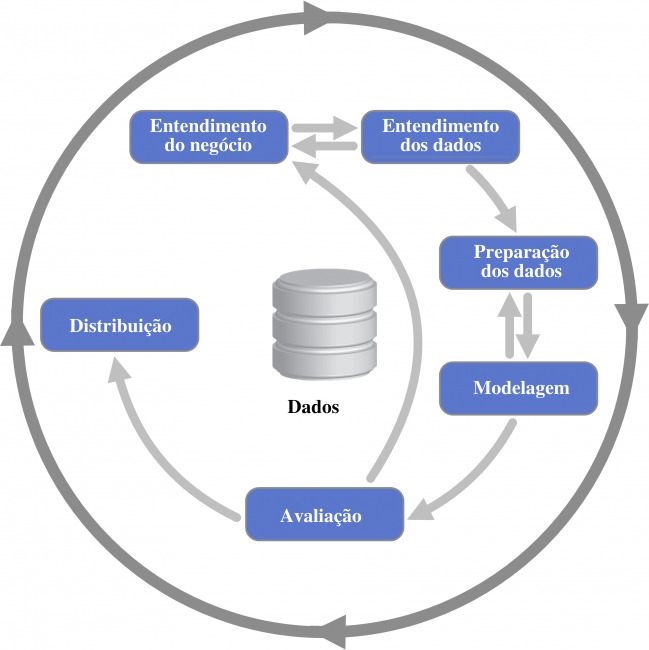
\includegraphics[scale=0.35]{figs/Ciclo de vida CRISP-DM.png}
    \caption{Ciclo de vida CRISP-DM.}
    \label{fig:ciclodevida}
\end{figure}

\begin{enumerate}
    \item \textbf{Compreensão do Negócio (\textit{Business Understanding}):} Nesta fase inicial, o foco consiste em compreender os objetivos e requisitos sob uma perspectiva operacional \cite{wirth2000crisp}. O conhecimento adquirido foi convertido em um problema formal de mineração de dados, ou seja, o desenvolvimento de um modelo de classificação supervisionado que utiliza os microdados da Subamostra Laboratorial da PNS 2013 \cite{IBGE_PNS2013_Exames}, cuja função é identificar indivíduos com perfis associados à hiperglicemia crônica clinicamente significativa, definida pelo critério laboratorial de HbA1c $\geq$ 6,5\%, conforme a reformulação conceitual do desfecho apresentada ao final desta seção.

    \item \textbf{Compreensão dos Dados (\textit{Data Understanding}):} Nesta fase, foi realizada a extração dos microdados da Subamostra Laboratorial da Pesquisa Nacional de Saúde, seguida de uma Análise Exploratória de Dados (EDA), a fim de mapear a distribuição das variáveis sociodemográficas, antropométricas e biológicas \cite{morgenthaler2009exploratory}, identificar correlações entre as variáveis e quantificar os valores ausentes e as anomalias presentes na amostra \cite{sahoo2019exploratory}. Na etapa descritiva, a prevalência do desfecho foi estimada também de forma ponderada pelo \textit{Peso\_Lab}, conforme descrito na seção de Base de Dados e Amostra Analítica. Os achados desta etapa subsidiaram as decisões sobre a seleção das variáveis de classificação e sobre o tratamento dos valores ausentes.

   \item \textbf{Preparação dos Dados (\textit{Data Preparation}):} Com base na análise exploratória, os dados foram submetidos a um \textit{pipeline} sequencial de preparação, estruturado a fim de prevenir qualquer forma de vazamento de informação (\textit{data leakage}) entre os subconjuntos de treino e teste. Inicialmente, o conjunto de dados foi dividido em treino (80\%) e teste (20\%), preservando a proporção da variável-alvo nos dois subconjuntos. Todas as etapas que aprendem parâmetros a partir dos dados, como a imputação de valores ausentes por meio do algoritmo \textit{K-Nearest Neighbors} (KNN) e a padronização das variáveis contínuas, foram ajustadas exclusivamente sobre o conjunto de treino e posteriormente aplicadas ao conjunto de teste, evitando assim a contaminação deste \cite{pedregosa2011scikit}. O detalhamento destas etapas é apresentado na seção de Preparação dos Dados, e o tratamento do desbalanceamento de classes, realizado por meio de aprendizagem sensível ao custo (\textit{Cost-Sensitive Learning}), é apresentado na seção de Tratamento do Desbalanceamento.

    \item \textbf{Modelagem (\textit{Modeling}):} Os microdados processados serviram de base para o treinamento de dois algoritmos de classificação supervisionada, implementados por meio da linguagem Python e da biblioteca \textit{scikit-learn} \cite{pedregosa2011scikit}. O primeiro algoritmo foi a Regressão Logística, utilizada como \textit{baseline} interpretável em virtude de sua transparência paramétrica e da consolidação histórica em estudos epidemiológicos \cite{nusinovici2020logistic}. O segundo foi o \textit{Random Forest}, escolhido em virtude de sua robustez frente à presença de variáveis correlacionadas, de sua capacidade de modelar interações não lineares entre as variáveis e de sua compatibilidade com técnicas de explicabilidade baseadas em valores de Shapley \cite{salih2025perspective}, cujos hiperparâmetros foram definidos por meio de uma busca descrita na seção de Modelagem. Seguindo o fluxo iterativo do CRISP-DM \cite{wirth2000crisp}, os achados desta fase motivaram retornos à fase de preparação dos dados, a exemplo do diagnóstico de multicolinearidade, que levou à remoção de uma variável e ao descarte de um dos conjuntos de atributos avaliados.

    \item \textbf{Avaliação (\textit{Evaluation}):} Os modelos desenvolvidos foram submetidos a um protocolo de avaliação em duas etapas. No conjunto de treino, a Validação Cruzada Estratificada com $k = 5$ \textit{folds} \cite{pertiwi2020comparison} foi utilizada para definir o limiar de decisão de cada modelo e para medir a variação das métricas entre partições \cite{pedregosa2011scikit}. No conjunto de teste, os modelos foram avaliados por meio de métricas derivadas da Matriz de Confusão \cite{Swaminathan2024}, tendo a Sensibilidade (\textit{Recall}) como métrica prioritária em virtude do contexto clínico de triagem, acompanhada da Especificidade, do \textit{F1-Score} e da Área Sob a Curva ROC (AUC-ROC) \cite{fawcett2006introduction, powers2020evaluation}. A essas métricas, previstas no projeto de pesquisa, somaram-se métricas complementares, a calibração das probabilidades e a comparação com uma regra clínica de rastreamento, de maneira que fosse possível identificar a estratégia mais adequada à tarefa de triagem proposta. O protocolo completo é apresentado na seção de Avaliação.

   \item \textbf{Implantação (\textit{Deployment}):} A fase de implantação compreende o painel de resultados, desenvolvido por meio do \textit{framework} Streamlit, e a disponibilização do modelo de referência por meio de uma API construída com o \textit{framework} FastAPI \cite{ramirez2018fastapi}, ambos descritos no capítulo de Desenvolvimento.
\end{enumerate}

\subsection{Reformulação Conceitual do Desfecho}
Para a operacionalização do desfecho do presente trabalho, fez-se necessária uma redefinição conceitual a partir das limitações intrínsecas da base de dados utilizada. A Subamostra Laboratorial da Pesquisa Nacional de Saúde (PNS) de 2013 não disponibiliza variável que diferencie clinicamente o Diabetes Mellitus tipo 1 (DM1) do tipo 2 (DM2), visto que o critério diagnóstico laboratorial de Hemoglobina Glicada (HbA1c) $\geq 6,5$\%, estabelecido pela American Diabetes Association \cite{ADA2010}, identifica a presença de hiperglicemia crônica independentemente do mecanismo patogênico subjacente.
Diante disso, o desfecho modelado por esta pesquisa foi reformulado como a presença de hiperglicemia crônica clinicamente significativa em adultos, operacionalizada por HbA1c $\geq$ 6,5\%, em detrimento da tentativa de discriminação diagnóstica entre subtipos de DM. Essa decisão metodológica sustenta-se em quatro fundamentos.
Em primeiro lugar, a literatura epidemiológica internacional indica que, entre adultos com diagnóstico de diabetes, mais de 90\% dos casos correspondem ao DM2 \cite{who2024diabetes}. No escopo nacional, o cenário não é diferente, visto que, segundo o Ministério da Saúde, cerca de 90\% dos pacientes diabéticos no Brasil possuem DM2 \cite{brasil2024diabetes}.

Em segundo lugar, no contexto da APS, a função do mecanismo de triagem proposto não consiste na discriminação diferencial entre subtipos de diabetes, mas sim na identificação precoce de indivíduos com perfis associados à hiperglicemia clinicamente significativa, gerando, por consequência, o encaminhamento para investigação laboratorial complementar \cite{brasil2013}. Logo, a responsabilidade da classificação etiológica específica é alocada à etapa subsequente do fluxo assistencial, conduzida por profissional médico em âmbito especializado.

Em terceiro lugar, as variáveis operacionalizadas pelo modelo correspondem predominantemente a determinantes associados ao DM2, tanto de natureza biológica, como a idade, a adiposidade e a hipertensão arterial sistêmica \cite{mlynarska2025type}, quanto de natureza social, como a escolaridade e a região \cite{deAlmeida-Pititto09112015}. Diante disso, os casos residuais de DM1 presentes na subamostra atuam como ruído no rótulo do desfecho, cuja proporção é limitada pela própria distribuição dos subtipos da doença, visto que cerca de 90\% dos casos de diabetes correspondem ao DM2 \cite{who2024diabetes, brasil2024diabetes}. Logo, admite-se que esse ruído, por representar uma fração minoritária dos casos positivos, não altera de forma expressiva as associações aprendidas pelos algoritmos, sendo este um pressuposto do presente trabalho e não uma garantia demonstrada empiricamente.

Em quarto lugar, há precedente direto na literatura que utiliza a própria PNS 2013 com critério laboratorial, visto que \textcite{muzy2021prevalencia}, ao estimar a prevalência de diabetes a partir da HbA1c da Subamostra Laboratorial, assumiram que a totalidade dos casos correspondia ao DM2, em virtude de 90\% a 95\% dos casos de diabetes serem desse tipo, corroborando a reformulação adotada neste trabalho.

\section{Seleção de Variáveis}\label{sec:selecao-variaveis}

\subsection{Princípios Orientadores}\label{sec:principios}
A seleção do conjunto de variáveis de classificação foi conduzida a partir de quatro princípios norteadores, estabelecidos com o objetivo de garantir a viabilidade científica, clínica e operacional do modelo proposto.

Pelo primeiro princípio, de não invasividade, foi priorizada a seleção exclusiva de variáveis obtidas por meio de entrevista, medição antropométrica ou aferição clínica não invasiva, a fim de viabilizar a aplicação do modelo no contexto da APS, no qual procedimentos laboratoriais representam, muitas vezes, barreiras estruturais e financeiras para a triagem populacional sistemática \cite{geremia2020atenccao}.

O segundo princípio, de compatibilidade com os sistemas de informação existentes, restringiu a composição do conjunto final às variáveis rotineiramente capturadas pelo Prontuário Eletrônico do Cidadão (PEC) no âmbito do Sistema de Informação em Saúde para a Atenção Básica (SISAB) \cite{brasil_esus_aps}, de maneira que, em trabalhos futuros, a metodologia desenvolvida apresente potencial de integração às bases de dados já consolidadas na rede pública brasileira sem exigência de coleta de novos dados ou alteração expressiva do fluxo assistencial.

O terceiro princípio, de robustez contra causalidade reversa, foi particularmente sensível em virtude da natureza transversal da PNS 2013 \cite{rothman2008modern}. Variáveis comportamentais estão sujeitas a alteração sistemática pós-diagnóstico de diabetes \cite{dimova2020diagnosis}, em especial a prática de exercício físico e o padrão alimentar, visto que as orientações clínicas posteriores ao diagnóstico prescrevem a inclusão ou o aumento da atividade física e a melhora da alimentação \cite{brasil2013}. Essas variáveis foram deliberadamente excluídas do conjunto final, a fim de mitigar a introdução de vieses de causalidade reversa no processo de aprendizagem do algoritmo. Caso mantidas, tais variáveis poderiam induzir o modelo a aprender regras estatisticamente invertidas, nas quais a presença de comportamento saudável se associa positivamente à condição patológica.

O quarto princípio, de parcimônia estatística e interpretabilidade, orientou a priorização de variáveis conceitualmente ortogonais, evitando redundância excessiva que dilua a interpretabilidade das contribuições individuais via SHAP (SHapley Additive exPlanations), cuja função é proporcionar a visualização do peso relativo de cada variável na classificação individual realizada pelo modelo \cite{salih2025perspective}.

\subsection{Variáveis Candidatas}\label{sec:variaveis-candidatas}
O conjunto de variáveis candidatas é composto por dezesseis variáveis, sendo quatorze obtidas diretamente dos microdados ou derivadas registro a registro e duas compostas, organizadas em cinco blocos temáticos, conforme apresentado a seguir. A composição de cada conjunto de atributos efetivamente utilizado no treinamento, a partir dessas candidatas, é apresentada na subseção de Conjuntos de Atributos.

Os códigos alfanuméricos dispostos entre parênteses ao longo desta seção, exemplo (C008), (Z001) e (W00303), correspondem aos identificadores oficiais de cada variável presentes no dicionário de microdados da Subamostra Laboratorial da Pesquisa Nacional de Saúde (PNS) de 2013, disponibilizado pelo IBGE \cite{IBGE_PNS2013_Exames}. A sua inclusão tem como objetivo viabilizar a rastreabilidade e a reprodutibilidade do estudo, de maneira que pesquisadores que venham a utilizar a mesma base de dados possam localizar com precisão cada variável operacionalizada no presente trabalho.

\begin{itemize}
\item[] \textbf{Variáveis Antropométricas e Biológicas: }
A inclusão das variáveis idade (C008) e sexo (Z001) fez-se necessária em virtude do papel determinante do envelhecimento na deterioração funcional das células beta pancreáticas e da sarcopenia progressiva \cite{mlynarska2025type}, bem como da prevalência diferenciada do DM2 entre sexos constatada em estudos populacionais brasileiros \cite{deAlmeida-Pititto09112015,muzy2021prevalencia,reis2022evolution}. O Índice de Massa Corporal (IMC) foi computado como variável derivada a partir da razão entre o peso final (z004) e o quadrado da altura final (z005), seguindo a fórmula clássica de Quetelet, cuja função é abranger a magnitude geral do acúmulo de tecido adiposo como indicador basal de resistência à insulina \cite{mlynarska2025type}. O peso e a altura foram utilizados apenas no cálculo das variáveis derivadas, não sendo fornecidos diretamente aos algoritmos, a fim de evitar que a mesma informação entrasse no modelo por canais redundantes.

A Circunferência da Cintura (W00303) foi incorporada em virtude da superioridade classificatória da adiposidade visceral sobre a adiposidade subcutânea generalizada, conforme fundamentado no referencial teórico. Diante disso, a utilização isolada do IMC como critério de triagem configura-se insuficiente para a identificação de perfis de risco metabólico relevantes na população adulta, de maneira que a mensuração complementar da circunferência da cintura torna-se necessária para a classificação dos perfis. A aferição desta variável na Subamostra Laboratorial da PNS 2013 seguiu o protocolo padronizado pelo IBGE, segundo o qual a medição foi realizada no ponto médio entre a borda inferior da última costela e a borda superior da crista ilíaca \cite{ibge2013pns}. A manutenção dessa variável em sua forma absoluta, mensurada em centímetros, se justifica pela existência de pontos de corte clinicamente consolidados para esse protocolo de aferição específico (circunferência $\geq 80$ cm para mulheres e $\geq 94$ cm para homens) \cite{SBD2019}.

Complementarmente, a Razão Cintura-Estatura (RCEst), derivada a partir da divisão entre Circunferência da Cintura (W00303) e altura final (z005), foi incluída como variável auxiliar, cujo papel é capturar a adiposidade visceral ajustada pela estatura individual, dimensão que não é abrangida de forma integral pelo IMC ou pela CC absoluta isoladamente \cite{Feller2010}. Diante disso, o bloco antropométrico candidato reúne três variáveis complementares sobre o fenótipo corporal do indivíduo, cuja permanência no modelo final foi condicionada ao diagnóstico descrito na seção de Tratamento da Multicolinearidade.

\item[] \textbf{Variáveis de Pressão Arterial Sistêmica: }
A Pressão Arterial Sistólica (W00407) e a Pressão Arterial Diastólica (W00408) foram incorporadas em suas formas contínuas aferidas objetivamente durante a coleta da PNS 2013 \cite{ibge2013pns}. A inclusão das medidas objetivas, em detrimento do uso exclusivo do autorrelato de HAS, é metodologicamente coerente com a premissa central deste trabalho, a qual preconiza a utilização de dados objetivos como critério superior ao autorrelato, em razão do fenômeno amplamente documentado de subnotificação diagnóstica na população brasileira \cite{muzy2021prevalencia,reis2022evolution,deAlmeida-Pititto09112015}.
 Adicionalmente, a variável HAS autorrelatada (Q002) foi mantida, com o objetivo de capturar a dimensão de consciência diagnóstica do indivíduo, variável esta que se comporta como proxy de acesso prévio ao sistema de saúde e de letramento em saúde. A partir da combinação destas duas fontes de informação, foi construída a variável derivada HAS Combinada, operacionalizada como positiva quando a pressão sistólica aferida é igual ou superior a 140 mmHg ou a diastólica é igual ou superior a 90 mmHg, conforme as diretrizes da Sociedade Brasileira de Diabetes \cite{SBD2019}, ou quando o autorrelato de diagnóstico é afirmativo, desconsiderando-se o relato de hipertensão exclusivamente durante a gravidez, de maneira que o modelo possa abranger tanto hipertensos previamente diagnosticados quanto hipertensos não diagnosticados, característica relevante para uma ferramenta de triagem que visa justamente identificar indivíduos em situação de vulnerabilidade clínica oculta.

\item[] \textbf{Diagnósticos Prévios Autorrelatados: }
O diagnóstico autorrelatado de colesterol alto (Q060) foi incorporado em virtude do papel consolidado da dislipidemia na Síndrome Metabólica, conforme fundamentado no referencial teórico.
Adicionalmente, foi desenvolvida a variável derivada \textit{Multimorbidade Metabólica}, operacionalizada como escore ordinal de zero a três, a partir da soma de três condições clínicas: HAS Combinada positiva; autorrelato afirmativo de colesterol alto (Q060); e presença de obesidade, definida pela ocorrência de IMC $\geq$ 30 kg/m² ou de Circunferência da Cintura $\geq$ 80 cm em mulheres ou $\geq$ 94 cm em homens \cite{SBD2019}. 
A escolha pela operacionalização disjuntiva do componente de obesidade, de maneira que a evidência por qualquer um dos dois indicadores antropométricos seja suficiente para a ativação do componente, fez-se necessária em virtude da limitação reconhecida do IMC isolado para a identificação de adiposidade central, conforme evidenciado na literatura \cite{Feller2010}.
O agrupamento de comorbidades metabólicas em um escore único busca viabilizar a captura de interações sinérgicas entre condições clínicas que, isoladamente, poderiam não atingir o limiar identificável pelos algoritmos, mas que, conforme a literatura especializada, em combinação elevam expressivamente a probabilidade de hiperglicemia crônica clinicamente significativa \cite{SBD2019,rzewuska2017epidemiology}.

\item[] \textbf{Variáveis Sociodemográficas: }
A raça/cor (Z003), a escolaridade (VDD004) e a posse de plano de saúde (I001) foram incorporadas como determinantes sociais da saúde, visto que, conforme o levantamento bibliográfico, estas variáveis atuam como \textit{proxies} das iniquidades históricas, do letramento em saúde e do acesso diferencial à rede assistencial brasileira \cite{deAlmeida-Pititto09112015,muzy2021prevalencia,reis2022evolution}. A raça/cor, em particular, foi interpretada neste trabalho exclusivamente como marcador de determinação social e de acesso aos serviços de saúde, e não como variável biológica.
A variável região (regiao) abrange a dimensão da heterogeneidade territorial brasileira, visto que a literatura constatou disparidades expressivas na prevalência e na subnotificação do DM2 entre as cinco macrorregiões do país \cite{muzy2021prevalencia,deAlmeida-Pititto09112015,reis2022evolution}.

\item[] \textbf{Autopercepção de Saúde: }
O estado de saúde autoavaliado (N001) foi mantido no conjunto final apesar de sua natureza subjetiva, em virtude da consolidação desta variável como indicador associado a desfechos crônicos em estudos epidemiológicos transversais e longitudinais, conforme descrito no referencial teórico \cite{Rantanen2019}. 
\end{itemize}

\subsection{Conjuntos de Atributos}\label{sec:conjuntos-atributos}
A partir das variáveis candidatas, foram construídos três conjuntos de atributos, cuja função é avaliar, por meio de experimentação, o efeito da redundância entre variáveis sobre o desempenho e a interpretabilidade dos modelos, em conformidade com o protocolo de tratamento da multicolinearidade previsto no projeto de pesquisa e com o quarto princípio orientador da seleção de variáveis. A composição de cada conjunto é apresentada no Quadro~\ref{qua:conjuntos}.

\begin{quadro}[htb]
  \caption{\label{qua:conjuntos}Conjuntos de atributos avaliados.}
  \small
  \begin{tabular}{|p{2.2cm}|p{6.2cm}|c|p{4.2cm}|}
    \hline
    \textbf{Conjunto} & \textbf{Variáveis} & \textbf{Colunas} & \textbf{Papel} \\ \hline
    A, atômico & Idade, IMC, CC, PAS, PAD, escolaridade, autopercepção de saúde, sexo, plano de saúde, raça/cor, região, HAS autorrelatada e colesterol alto & 20 & Componentes isolados, sem escores agregados \\ \hline
    B, composto & Idade, IMC, CC, escolaridade, autopercepção de saúde, Multimorbidade Metabólica, sexo, plano de saúde, raça/cor e região & 16 & Escore de multimorbidade no lugar das pressões e dos diagnósticos autorrelatados \\ \hline
    C, completo & As dezesseis candidatas, incluindo RCEst, HAS Combinada e Multimorbidade Metabólica & 23 & Componentes e escores simultaneamente \\ \hline
  \end{tabular}
  \fonte{Elaborado pelo autor.}
\end{quadro}

Na coluna ``Colunas'', considera-se o número de colunas da matriz de dados fornecida aos algoritmos, após a codificação das variáveis nominais. A diferença entre os conjuntos reside no grau de ortogonalidade entre essas colunas, avaliado em dois níveis. No nível estrito, nenhuma variável de origem entra no modelo, ao mesmo tempo, como coluna própria e como parcela idêntica de uma variável agregada, condição atendida pelos conjuntos A e B. No nível pleno, nenhuma variável de origem contribui para o modelo por mais de um caminho, em qualquer forma, condição atendida apenas pelo conjunto A. Esses dois níveis foram verificados por testes automatizados sobre a proveniência de cada coluna, descritos no capítulo de Desenvolvimento.

No conjunto B, permanece uma sobreposição residual, visto que o IMC, a circunferência da cintura e o sexo entram como colunas próprias e também alimentam o componente de obesidade do escore de multimorbidade, porém em forma binarizada por ponto de corte clínico, de maneira que o gradiente contínuo dessas variáveis carrega uma informação que o limiar descarta. Pelo mesmo motivo de ortogonalidade, a HAS Combinada, que constitui a primeira parcela do escore, foi mantida fora do conjunto B, a fim de que o modelo não recuperasse a parcela diretamente e a hipótese de sinergia entre as condições clínicas permanecesse testável. Já o conjunto C repete deliberadamente a mesma informação por mais de um canal, a exemplo da HAS autorrelatada e do colesterol alto, que entram como colunas próprias e novamente dentro do escore, com o objetivo de quantificar o custo dessa redundância. Por fim, a RCEst integra apenas o conjunto C, visto que sua exclusão dos conjuntos A e B decorreu do diagnóstico descrito na seção de Tratamento da Multicolinearidade, cujos valores são apresentados no capítulo de Resultados.

\section{Preparação dos Dados}\label{sec:preparacao}

\subsection{Particionamento}\label{sec:particionamento}
A amostra analítica foi dividida em um conjunto de treino, com 80\% dos registros, e um conjunto de teste, com os 20\% restantes, por meio de amostragem estratificada pela variável-alvo, de maneira que a proporção de casos positivos fosse preservada nos dois subconjuntos \cite{pedregosa2011scikit}. Nenhuma operação que dependesse de mais de um registro foi executada antes dessa divisão, a fim de que nenhuma informação do conjunto de teste influenciasse qualquer etapa do treinamento. Diante disso, toda etapa que aprende parâmetros a partir dos dados, como a imputação, a padronização e a codificação das variáveis, foi ajustada exclusivamente sobre o conjunto de treino e apenas aplicada ao conjunto de teste. Todas as operações estocásticas do trabalho, incluindo a divisão dos dados, utilizaram a mesma semente aleatória, de valor 42, a fim de garantir a reprodutibilidade dos resultados.

\subsection{Imputação de Valores Ausentes}\label{sec:imputacao}
Os valores ausentes das variáveis classificadoras foram imputados por meio do algoritmo \textit{K-Nearest Neighbors} (KNN), conforme previsto no projeto de pesquisa, utilizando cinco vizinhos ponderados pelo inverso da distância \cite{pedregosa2011scikit}. A variável-alvo não foi imputada, visto que os registros sem valor válido de HbA1c já haviam sido excluídos da amostra analítica. A imputação foi posicionada como a primeira etapa do \textit{pipeline} de preparação e aplicada sobre todas as variáveis candidatas, e não apenas sobre as colunas de cada conjunto de atributos, em virtude de as variáveis compostas, construídas na etapa seguinte, dependerem de componentes que nem todos os conjuntos utilizam como coluna própria.

Como o KNN seleciona os vizinhos por meio da distância euclidiana, a aplicação direta do algoritmo sobre as variáveis em suas escalas originais faria com que as variáveis de maior amplitude numérica, como a pressão arterial e a idade, dominassem a seleção dos vizinhos. Diante disso, o espaço de distância foi restrito às variáveis contínuas, padronizadas por meio de um ajuste realizado apenas sobre o conjunto de treino, e à variável sexo, por ser binária e, portanto, a única variável categórica em que a distância possui significado direto. As demais variáveis categóricas, como raça/cor, região e escolaridade, não participaram do cálculo da distância, visto que a diferença numérica entre seus códigos não representa uma diferença real entre categorias, porém permaneceram como alvo da imputação. Os valores imputados dessas variáveis foram arredondados para o código válido mais próximo entre os observados no treino, de maneira que a codificação posterior permanecesse consistente. Por fim, as variáveis contínuas foram devolvidas à sua escala clínica original após a imputação, visto que as variáveis compostas utilizam pontos de corte expressos em unidades reais.

\subsection{Variáveis Derivadas}\label{sec:derivadas}
As variáveis derivadas foram construídas em dois momentos distintos, conforme dependessem ou não de informações de outros registros. O IMC, calculado pela razão entre o peso em quilogramas e o quadrado da altura em metros, e a RCEst, calculada pela razão entre a circunferência da cintura e a altura, foram construídos registro a registro durante a limpeza dos dados, visto que dependem apenas das medidas do próprio indivíduo. Já as variáveis compostas, isto é, a HAS Combinada e a Multimorbidade Metabólica, foram construídas dentro do \textit{pipeline}, após a imputação, em virtude de dependerem de componentes imputados, cujo ajuste é realizado apenas sobre o conjunto de treino. A construção dessas variáveis antes da divisão dos dados faria com que o conjunto de teste carregasse uma imputação ajustada sobre a base completa, configurando vazamento de informação. Nesta mesma etapa, as variáveis sexo, posse de plano de saúde e colesterol alto foram recodificadas como indicadoras binárias.

Na última etapa do \textit{pipeline}, cada conjunto de atributos selecionou as suas colunas, sobre as quais foram aplicadas a padronização das variáveis numéricas, a manutenção das variáveis binárias em sua forma original e a codificação das variáveis nominais em variáveis indicadoras, omitindo-se uma categoria de referência por variável \cite{pedregosa2011scikit}. Por consequência dessa omissão, a categoria de referência de cada variável nominal não possui coluna própria, característica que influencia a leitura da explicabilidade, conforme descrito na seção de Explicabilidade.

\section{Tratamento da Multicolinearidade}\label{sec:trat-multicolinearidade}

A manutenção simultânea de variáveis antropométricas correlacionadas (IMC, CC e RCEst) e de múltiplas variáveis de pressão arterial configurou um cenário de multicolinearidade que demandou tratamento metodológico específico, conforme apresentado no referencial teórico. A fim de diagnosticar esse problema, foram computados, sobre o conjunto de treino, os coeficientes de correlação de Pearson entre as variáveis contínuas e os Fatores de Inflação de Variância (VIF) de cada coluna \cite{Senaviratna2019}. O VIF foi calculado sobre a matriz de dados completa fornecida aos algoritmos, isto é, após a padronização e a codificação das variáveis nominais, de maneira que as variáveis binárias e as indicadoras também fossem incluídas no diagnóstico. Ao lado de cada VIF, foi reportado o coeficiente de determinação ($R^2$) da regressão auxiliar correspondente, obtido por $R^2 = 1 - 1/\text{VIF}$, visto que este expressa diretamente a fração da variância de uma coluna já explicada pelas demais.

O protocolo foi orientado pelo limiar convencional de VIF $> 10$ \cite{Senaviratna2019}. Para as variáveis de um mesmo bloco temático que excederam esse limiar, a variável de maior VIF foi removida de forma experimental e o diagnóstico foi recalculado, a fim de verificar se a remoção resolvia a violação ou se a redundância persistia nas demais colunas. No que se refere ao \textit{Random Forest}, a multicolinearidade não compromete o desempenho classificatório do algoritmo \cite{Chan2022}, de maneira que o tratamento nesse modelo foi direcionado ao plano da interpretabilidade, conforme descrito na seção de Explicabilidade.

Adicionalmente, a redundância entre o escore de Multimorbidade Metabólica e os seus componentes foi avaliada por um teste complementar ao VIF. Como o escore é obtido pela soma de três parcelas, das quais uma, o componente de obesidade, decorre da aplicação de pontos de corte sobre o IMC e a circunferência da cintura, a dependência entre o escore e as colunas contínuas não é linear e não pode ser integralmente capturada pela regressão auxiliar do VIF. Diante disso, o escore foi regredido diretamente sobre as suas três parcelas, de maneira que um coeficiente de determinação igual a um indicasse que o escore não acrescenta nenhuma informação ausente de seus componentes. Este teste não estava previsto no projeto de pesquisa e foi acrescentado em virtude dessa limitação estrutural do VIF diante de variáveis construídas por ponto de corte.

\section{Tratamento do Desbalanceamento}\label{sec:desbalanceamento}

Em virtude da baixa prevalência do desfecho na amostra, o desbalanceamento entre as classes foi tratado por meio de aprendizagem sensível ao custo, conforme previsto no projeto de pesquisa, em detrimento de técnicas de reamostragem como o SMOTE, cuja geração de observações sintéticas é incompatível com a estrutura de ponderação amostral da PNS 2013, conforme discutido no referencial teórico \cite{araf2024costsensitive, 10.1371/journal.pone.0280387}. Nenhum registro foi criado, removido ou duplicado para equilibrar as classes, visto que a estratégia adotada atua sobre a função de perda dos algoritmos, atribuindo maior peso aos erros de classificação da classe minoritária.

Na Regressão Logística, essa estratégia foi implementada por meio do hiperparâmetro \texttt{class\_weight='balanced'}, que atribui a cada classe um peso inversamente proporcional à sua frequência no conjunto de treino \cite{pedregosa2011scikit}. No \textit{Random Forest}, foi utilizada a variante \texttt{class\_weight='balanced\_subsample'}, na qual o mesmo cálculo é refeito sobre a amostra \textit{bootstrap} de cada árvore \cite{sklearn2026randomforest}. A atribuição de pesos distintos por classe em florestas aleatórias é uma abordagem estudada para o processamento de dados médicos desbalanceados, com melhora na identificação da classe minoritária \cite{zhu2018classweights}.

O projeto de pesquisa nomeava literalmente o valor \texttt{balanced} para os dois algoritmos, de maneira que a adoção da variante por subamostra na floresta constitui uma divergência formal em relação ao texto assinado, porém não em relação ao método nele estabelecido, visto que ambos os valores implementam a aprendizagem sensível ao custo e nenhum deles cria observações sintéticas. A diferença reside no fato de que, em uma floresta, cada árvore é ajustada sobre uma reamostragem do treino com distribuição de classes própria, de maneira que o valor \texttt{balanced} aplica, dentro de cada árvore, pesos calculados sobre uma distribuição que não é a dela, enquanto o \texttt{balanced\_subsample} recalcula os pesos sobre a amostra que a árvore efetivamente utiliza. Diante disso, considerou-se o \texttt{balanced\_subsample} como a forma, em uma floresta, do que o \texttt{balanced} realiza na Regressão Logística, a qual não possui reamostragem interna. Os dois valores foram avaliados na busca de hiperparâmetros, descrita na seção de Modelagem.

Por fim, o reponderamento das classes possui uma consequência sobre as probabilidades produzidas pelos modelos. \textcite{vandengoorbergh2022harm} demonstraram que métodos de correção do desbalanceamento produzem modelos mal calibrados, com superestimação sistemática da probabilidade da classe minoritária e sem ganho de capacidade discriminativa, e que o deslocamento do limiar de decisão produz efeito semelhante sobre a sensibilidade e a especificidade. Embora o estudo tenha avaliado métodos de reamostragem, o reponderamento altera da mesma forma a distribuição de classes que o algoritmo considera durante o ajuste, de maneira que o mesmo efeito era esperado neste trabalho, tendo sido verificado empiricamente, conforme apresentado no capítulo de Resultados. Por consequência, a classificação dos indivíduos foi realizada por meio de um limiar de decisão calibrado, descrito na seção de Ponto de Operação, e as probabilidades produzidas pelos modelos não foram interpretadas como risco individual.

\section{Modelagem}\label{sec:modelagem}

A modelagem compreendeu o treinamento de dois algoritmos sobre os conjuntos de atributos descritos anteriormente, ambos encapsulados em um mesmo \textit{pipeline} junto das etapas de preparação, de maneira que toda transformação fosse reajustada a cada treinamento, utilizando apenas os dados de treino disponíveis naquele momento. A Regressão Logística foi treinada nos três conjuntos de atributos, enquanto o \textit{Random Forest} foi treinado apenas nos conjuntos A e B, visto que o conjunto C foi descartado pelo diagnóstico de multicolinearidade, permanecendo na Regressão Logística como evidência empírica desse descarte.

\subsection{Regressão Logística}\label{sec:logistica}
A Regressão Logística foi configurada com o reponderamento de classes descrito na seção de Tratamento do Desbalanceamento e com um limite de 1.000 iterações para a convergência do algoritmo de otimização, mantendo-se a regularização padrão da biblioteca \cite{pedregosa2011scikit}. Não foi realizada busca de hiperparâmetros para este algoritmo, visto que a sua configuração decorre de decisões metodológicas previstas no projeto de pesquisa e de seu papel como \textit{baseline} interpretável.

\subsection{\textit{Random Forest} e Busca de Hiperparâmetros}\label{sec:random-forest}
Diferentemente da Regressão Logística, o \textit{Random Forest} possui hiperparâmetros que controlam diretamente a capacidade do modelo, como a profundidade máxima das árvores, o número mínimo de registros por folha e o número de variáveis avaliadas em cada divisão. O projeto de pesquisa não previa procedimento para a definição desses valores, e a manutenção dos valores padrão da biblioteca constituiria uma escolha implícita, na qual cada árvore cresce até que suas folhas contenham registros de uma única classe. Diante disso, os hiperparâmetros foram definidos por meio de uma busca aleatória \cite{pedregosa2011scikit}, na qual sessenta combinações foram sorteadas a partir do espaço apresentado no Quadro~\ref{qua:busca}, que também apresenta a configuração adotada.

\begin{quadro}[htb]
  \caption{\label{qua:busca}Espaço da busca de hiperparâmetros do \textit{Random Forest} e configuração adotada.}
  \small
  \begin{tabular}{|p{3.0cm}|p{4.4cm}|p{2.4cm}|p{4.4cm}|}
    \hline
    \textbf{Hiperparâmetro} & \textbf{Valores avaliados} & \textbf{Valor adotado} & \textbf{Função} \\ \hline
    \texttt{max\_depth} & Sem limite, 6, 10, 14 e 20 & 10 & Profundidade máxima de cada árvore \\ \hline
    \texttt{min\_samples\_leaf} & 5, 10, 20 e 40 & 20 & Número mínimo de registros em cada folha \\ \hline
    \texttt{max\_features} & Raiz quadrada e logaritmo na base 2 do número de colunas; 30\% e 50\% das colunas & Raiz quadrada & Quantidade de colunas avaliadas em cada divisão \\ \hline
    \texttt{class\_weight} & \texttt{balanced} e \texttt{balanced\_subsample} & \texttt{balanced\_ subsample} & Forma do reponderamento das classes \\ \hline
    \texttt{n\_estimators} & Fixo, fora da busca & 500 & Número de árvores da floresta \\ \hline
  \end{tabular}
  \fonte{Elaborado pelo autor.}
\end{quadro}

O número de árvores foi fixado em quinhentas, fora do espaço de busca, visto que este parâmetro afeta a estabilidade da agregação e não a capacidade do modelo. O número mínimo de registros por folha teve como menor valor avaliado cinco registros, a fim de evitar folhas com um único registro, que produzem probabilidades quase degeneradas e prejudicam a definição posterior do limiar de decisão.

Cada combinação foi avaliada por Validação Cruzada Estratificada com cinco partições sobre o conjunto de treino, na qual todo o \textit{pipeline}, incluindo a imputação, foi reajustado dentro de cada partição, de maneira que nenhuma partição de validação influenciasse o próprio pré-processamento. O conjunto de teste não participou da busca em nenhum momento.

A métrica de seleção foi a área sob a curva de precisão e sensibilidade (PR-AUC), calculada pela precisão média ao longo dos limiares \cite{Swaminathan2024}. A escolha decorre do fato de que o limiar de decisão de cada modelo é definido somente após a busca, de maneira que métricas dependentes de limiar, como a sensibilidade, seriam calculadas sobre o limiar padrão de 0,5, no qual o modelo não opera. Além disso, a curva de precisão e sensibilidade constitui alternativa à curva ROC para dados desbalanceados, nos quais a AUC-ROC pode induzir a interpretações equivocadas \cite{Swaminathan2024}. A sensibilidade permaneceu como a métrica prioritária na avaliação dos resultados, porém não na seleção dos hiperparâmetros.

A busca foi executada nos conjuntos A e B, com a mesma lista de combinações sorteadas para ambos, e a configuração vencedora no conjunto B foi aplicada aos dois conjuntos, a fim de que a comparação entre A e B isolasse o efeito do conjunto de atributos, sem misturá-lo a diferenças de configuração. Na comparação entre as duas formas de reponderamento, a busca não separou os valores, visto que a diferença de PR-AUC entre a melhor configuração de cada um foi inferior à dispersão entre as partições, conforme apresentado no capítulo de Resultados. Diante disso, a escolha do \texttt{balanced\_subsample} apoiou-se no argumento descrito na seção de Tratamento do Desbalanceamento, e não na diferença numérica.

\section{Avaliação}\label{sec:avaliacao-metodo}

\subsection{Ponto de Operação}\label{sec:ponto-operacao}
Em virtude do reponderamento das classes, o limiar padrão de 0,5 não corresponde a um ponto de operação adequado à baixa prevalência do desfecho, de maneira que o limiar de decisão de cada modelo foi tratado como um parâmetro explícito, definido a partir de uma sensibilidade-alvo. Para cada modelo, foram obtidas as probabilidades previstas para os registros de treino por meio de Validação Cruzada Estratificada com cinco partições, de modo que cada probabilidade fosse produzida por um modelo que não utilizou aquele registro em seu ajuste. Entre os limiares que atingiram a sensibilidade-alvo nessas probabilidades, foi escolhido o maior, visto que este mantém a mesma sensibilidade com o menor número de encaminhamentos. O conjunto de teste não participou da definição do limiar, procedimento que corresponde ao ajuste do limiar de decisão como método de tratamento do desbalanceamento no nível do algoritmo \cite{thabtah2020data} e que, conforme \textcite{vandengoorbergh2022harm}, produz sobre a sensibilidade e a especificidade efeito semelhante ao das técnicas de correção do desbalanceamento.

A sensibilidade-alvo foi fixada em 0,80, valor situado no limite superior da faixa de sensibilidade obtida pelo FINDRISC e por suas adaptações latino-americanas em seus pontos de corte recomendados, entre 0,667 e 0,73, com exceção de uma versão simplificada, que atingiu 0,859 \cite{CarrilloLarco2020}. Cabe destacar que os desfechos avaliados por esses instrumentos diferem do desfecho deste trabalho, de maneira que essa faixa foi utilizada apenas para estabelecer a ordem de grandeza do ponto de operação, e não como base de comparação de desempenho. A escolha de um ponto de operação implica uma troca entre a fração de casos detectados e a fração da população encaminhada a exame, conforme a avaliação de estratégias de rastreamento conduzida por \textcite{bracco2026brdmrisc}, o que se torna determinante em um contexto como o da APS, que opera predominantemente por demanda espontânea e com capacidade limitada \cite{geremia2020atenccao}. Por fim, a definição deste ponto de operação como principal foi registrada após o conhecimento dos resultados obtidos tanto neste ponto quanto no regime de comparação com a regra clínica, descrito adiante, razão pela qual os dois regimes são sempre reportados lado a lado.

\subsection{Métricas}\label{sec:metricas}
No conjunto de teste, cada modelo foi avaliado no seu limiar de decisão por meio das métricas previstas no projeto de pesquisa, isto é, a Sensibilidade, métrica prioritária, a Especificidade, o \textit{F1-Score} e a AUC-ROC, definidas no referencial teórico \cite{Swaminathan2024, fawcett2006introduction}. A acurácia não foi utilizada como critério, visto que, em dados desbalanceados, um classificador que atribui todos os indivíduos à classe majoritária obtém acurácia elevada sem identificar nenhum caso \cite{Swaminathan2024}.

A essas métricas, somaram-se três complementares, não previstas no projeto de pesquisa. A primeira foi a PR-AUC, mais informativa que a AUC-ROC em dados desbalanceados \cite{Swaminathan2024}, cujo valor de referência para um classificador sem capacidade discriminativa corresponde à prevalência da classe positiva, e não a 0,5. A segunda foi o número necessário para rastrear (NNS), calculado como o número de indivíduos encaminhados a exame para cada caso detectado, métrica utilizada pela própria diretriz brasileira de rastreamento para fundamentar a idade de início do rastreamento \cite{Rodacki2025}. A terceira foi a taxa de encaminhamento, calculada como a fração dos indivíduos avaliados que o modelo encaminha a exame, a fim de traduzir cada ponto de operação na carga gerada para a rede de saúde.

Ao lado de cada métrica obtida no conjunto de teste, foram reportados a média e o desvio padrão da mesma métrica entre as cinco partições da validação cruzada no treino, calculados no mesmo limiar de decisão. Essa dispersão fornece a escala para julgar se a diferença entre dois modelos ou dois conjuntos de atributos excede a variação esperada entre partições dos dados, sendo utilizada nos critérios de comparação descritos na seção de Comparadores e Critério de Sucesso.

\subsection{Calibração das Probabilidades}\label{sec:calibracao}
Em virtude do reponderamento das classes, as probabilidades produzidas pelos modelos foram avaliadas quanto à sua calibração, isto é, quanto à concordância entre a probabilidade prevista e a frequência observada do desfecho. O escore de Brier foi reportado como medida de desempenho global das probabilidades, a qual reúne discriminação e calibração \cite{vandengoorbergh2022harm}, acompanhado do escore de um previsor constante igual à prevalência do conjunto de teste e da razão entre os dois, denominada \textit{Brier skill}, cujo valor negativo indica desempenho inferior ao desse previsor.

A calibração propriamente dita foi avaliada por três instrumentos complementares, todos calculados sobre o conjunto de teste. O primeiro foi a curva de calibração por decis, na qual os registros foram ordenados pela probabilidade prevista e divididos em dez grupos de mesmo tamanho, comparando-se, em cada grupo, a probabilidade média prevista com a frequência observada do desfecho. O segundo foi o erro de calibração esperado (ECE), calculado como a média, ponderada pelo tamanho de cada grupo, da diferença absoluta entre essas duas quantidades \cite{guo2017calibration}, utilizando os mesmos decis, forma de agrupamento adaptativa discutida por \textcite{posocco2021ece}. O terceiro foi a regressão logística do desfecho observado sobre o logito das probabilidades previstas, da qual foram extraídos a inclinação e o intercepto de calibração, estimados conjuntamente e sem penalização, de maneira que um modelo perfeitamente calibrado apresentaria inclinação igual a um e intercepto igual a zero. Conforme \textcite{vandengoorbergh2022harm}, um intercepto negativo indica superestimação sistemática das probabilidades, e uma inclinação inferior a um indica probabilidades excessivamente extremas. Por fim, foi reportada a razão entre a probabilidade média prevista e a prevalência observada, que expressa quantas vezes os modelos superestimam, em média, a frequência do desfecho.

\subsection{Comparadores e Critério de Sucesso}\label{sec:comparadores}
O projeto de pesquisa discutia o FINDRISC e o BrDMrisc como referências para a triagem de DM2, porém nenhum dos dois pôde ser reproduzido sobre os dados deste trabalho. O FINDRISC depende do histórico familiar de diabetes e de variáveis comportamentais \cite{conceiccao2020translation}, excluídas pelo terceiro princípio orientador da seleção de variáveis, e o BrDMrisc estima o risco de diabetes incidente a partir de uma coorte longitudinal \cite{bracco2026brdmrisc}, desenho incompatível com o desenho transversal da PNS 2013. Diante disso, foram adotados dois comparadores não baseados em aprendizagem de máquina. O primeiro foi uma regra clínica de rastreamento, que encaminha a exame todo indivíduo com idade igual ou superior a 35 anos ou com IMC igual ou superior a 25 kg/m², em conformidade com a idade de início do rastreamento universal e com o critério de excesso de peso adotados pela diretriz brasileira \cite{Rodacki2025}. A regra constitui uma simplificação da diretriz, visto que esta associa o excesso de peso a fatores de risco adicionais, dentre os quais o histórico familiar, excluído deste trabalho. O segundo comparador foi um classificador que atribui todos os indivíduos à classe majoritária, cuja função é marcar o desempenho mínimo de referência.

Como os dois comparadores produzem diretamente a decisão de encaminhar ou não, e não uma probabilidade, ambos foram avaliados com limiar fixo, sem a calibração de limiar aplicada aos modelos. Por consequência, as métricas que dependem da curva de probabilidades, como a AUC-ROC e a PR-AUC, não são comparáveis entre os comparadores e os modelos, sendo a comparação restrita à sensibilidade, à especificidade, ao NNS e à taxa de encaminhamento.

O critério de sucesso, estabelecido antes da execução e não previsto no projeto de pesquisa, foi superar a regra clínica em sensibilidade e, simultaneamente, apresentar NNS menor. Como a comparação de NNS entre estratégias que operam em sensibilidades diferentes não ordena essas estratégias, visto que encaminhar menos pessoas para detectar menos casos também reduz o NNS, o critério foi avaliado em um regime de sensibilidade equiparada, no qual o limiar de cada modelo foi recalibrado para atingir a sensibilidade que a regra obtém no conjunto de treino, e não no de teste, a fim de evitar o vazamento de informação do teste para a definição do limiar. O regime principal e o regime equiparado foram reportados lado a lado para todas as combinações de modelo e conjunto de atributos.

Por fim, três regras de comparação entre os modelos foram declaradas antes da execução dos experimentos. A primeira estabelece que a diferença entre dois modelos, ou entre dois conjuntos de atributos, que não exceda o desvio padrão entre as partições da validação cruzada é tratada como indistinguível, sendo a escolha, nesse caso, orientada pela parcimônia e pela interpretabilidade. A segunda estabelece que, havendo empate entre a Regressão Logística e o \textit{Random Forest} na sensibilidade do teste, a Regressão Logística é mantida como modelo principal. A terceira estabelece como modelo de referência, para a comparação com a regra clínica, a combinação de modelo e conjunto de atributos com o menor NNS no ponto de operação principal, aplicando-se a regra de parcimônia em caso de empate.

\subsection{Comparação Pareada entre Modelos}\label{sec:mcnemar}
A comparação entre a Regressão Logística e o \textit{Random Forest} foi complementada pelo teste de McNemar, aplicado sobre as classificações dos dois modelos para os mesmos indivíduos do conjunto de teste, cada modelo em seu próprio limiar de decisão. O teste considera apenas os pares discordantes, isto é, os indivíduos classificados corretamente por um modelo e incorretamente pelo outro, e foi calculado em sua versão exata condicional, baseada na distribuição binomial \cite{fagerland2013mcnemar}. Conforme \textcite{fagerland2013mcnemar}, essa versão é conservadora, isto é, tende a rejeitar a hipótese nula com frequência inferior ao nível de significância nominal, de maneira que um resultado não significativo deve ser lido com essa ressalva. Além do teste sobre todos os indivíduos, foi reportado o recorte restrito aos casos positivos, a fim de identificar se um dos modelos detecta casos que o outro não detecta. O teste foi acrescentado após a aplicação da regra de comparação entre os modelos e não a alterou, servindo apenas para qualificar a forma como a diferença entre eles é descrita.

\section{Explicabilidade}\label{sec:explicabilidade}

A explicabilidade dos modelos foi obtida por meio da biblioteca SHAP (\textit{SHapley Additive exPlanations}), abrangendo duas dimensões complementares de análise \cite{salih2025perspective}. A dimensão global, calculada sobre o conjunto de teste completo, quantifica a importância relativa de cada variável na composição agregada das classificações, enquanto a dimensão local decompõe a contribuição de cada variável no escore atribuído a um indivíduo. O projeto de pesquisa previa a aplicação do \textit{TreeExplainer} ao \textit{Random Forest} e do \textit{LinearExplainer} à Regressão Logística, porém a análise foi executada apenas sobre o \textit{Random Forest}, nos conjuntos de atributos A e B, permanecendo a explicabilidade da Regressão Logística como etapa não executada, conforme discutido nas limitações deste trabalho. Em ambas as dimensões, as contribuições expressam associações estatísticas observadas em dados transversais, não constituindo relações causais nem predições de desenvolvimento futuro da condição clínica avaliada.

Em virtude da multicolinearidade remanescente entre algumas variáveis, cujo efeito sobre o SHAP é discutido no referencial teórico, e como nenhum dos métodos de mitigação identificados por \textcite{Salih2024} elimina, por natureza, esse efeito sobre as explicações, a estratégia adotada foi construída especificamente para este trabalho, não constituindo aplicação de um método da literatura. Essa estratégia teve início antes da explicabilidade, com a remoção da RCEst e com o desenho dos conjuntos A e B, e foi complementada pela execução da análise em dois regimes de perturbação do \textit{TreeExplainer}, ambos sobre o conjunto de teste completo. O regime principal, denominado \textit{tree path dependent}, utiliza a cobertura das próprias árvores e, por consequência, respeita a dependência entre variáveis que o modelo efetivamente observou durante o treinamento, sendo sobre ele que se baseiam a importância global e as explicações locais apresentadas. O regime de contraste, denominado \textit{interventional}, assume independência entre as variáveis, utilizando como referência uma amostra de cem registros do conjunto de treino, e corresponde à formulação que a literatura aponta como frágil diante da multicolinearidade. Diante disso, a divergência entre os rankings de importância produzidos pelos dois regimes foi utilizada como medida da exposição deste trabalho ao problema.

A propriedade de aditividade, segundo a qual a soma das contribuições de um indivíduo reconstrói a saída do modelo, foi verificada em vez de presumida. No regime principal, a aditividade foi atendida com erro da ordem da precisão numérica do computador. No regime de contraste, a versão da biblioteca utilizada apresentou erros de aditividade em um subconjunto das árvores, localizados árvore a árvore, cuja origem é o algoritmo do explicador, e não o modelo, visto que as mesmas árvores são explicadas sem erro no regime principal. Diante disso, o regime de contraste foi calculado sobre uma floresta reduzida, obtida da mesma floresta ajustada pela exclusão das árvores com erro de aditividade superior a $10^{-4}$ sobre os registros explicados, de maneira que o contraste fosse exato. A floresta reduzida constitui um objeto de diagnóstico, e não um modelo publicado. A comparação entre os regimes foi definida antes da medição e realizada com os dois regimes aplicados à mesma floresta reduzida, a fim de isolar o efeito da troca de regime do efeito da remoção das árvores.

As atribuições foram reportadas em dois níveis. No primeiro, por coluna da matriz de dados, que corresponde ao que o modelo efetivamente utiliza; no segundo, por variável conceitual, somando-se as colunas indicadoras de uma mesma variável nominal. Em virtude da omissão de uma categoria de referência na codificação das variáveis nominais, descrita na seção de Variáveis Derivadas, a categoria de referência de cada variável nominal possui atribuição nula por construção, e não por irrelevância.

Além disso, três estruturas de dependência remanescentes nos conjuntos analisados foram nomeadas antes da medição: o par formado pelo IMC e pela circunferência da cintura, nos conjuntos A e B; o par de pressões sistólica e diastólica, no conjunto A; e o bloco formado pelo IMC, pela circunferência da cintura e pelo sexo em relação ao escore de Multimorbidade Metabólica, no conjunto B, em virtude do componente de obesidade do escore. As atribuições desses pares e blocos foram reportadas sempre em duas formas, individual e somada, lado a lado, sem limiar que decidisse pelo agrupamento, de maneira que a divisão do crédito entre membros correlacionados ficasse visível ao leitor.

Também antes da medição, foi registrada uma predição baseada no mecanismo descrito por \textcite{Salih2024}: dentro de cada par ou bloco, um dos membros concentraria a atribuição e o outro teria sua atribuição reduzida, sendo essa redistribuição mais acentuada no regime de contraste. Nenhuma decisão sobre o modelo dependeu do resultado dessa predição, visto que a explicabilidade foi utilizada para descrever o modelo publicado, e não para modificá-lo, de maneira que nenhuma variável foi removida, agrupada ou reordenada, e nenhum hiperparâmetro ou limiar foi alterado em função das atribuições.

A leitura das atribuições está sujeita a uma restrição decorrente do reponderamento das classes. As contribuições são expressas na escala da fração de votos da floresta, a mesma em que o limiar de decisão opera, de maneira que a soma das contribuições de um indivíduo reconstrói o seu escore de ordenação, e não o seu risco. Além disso, o valor de base das explicações, que corresponde à média das saídas do modelo, situa-se próximo de 0,5 em virtude do reponderamento, e não próximo da prevalência do desfecho. Por consequência, como a maior parte dos indivíduos recebe escores inferiores a esse valor, a explicação local de quase todo indivíduo é composta majoritariamente por contribuições negativas. Uma contribuição negativa indica, portanto, um valor abaixo da referência representada pelo indivíduo médio sob reponderamento de classes, e nunca um efeito protetor.

Para a dimensão local, foram selecionados, em cada conjunto de atributos, quatro casos do conjunto de teste, um de cada célula da matriz de confusão, sendo escolhido, em cada célula, o indivíduo com escore mais próximo do limiar de decisão. As explicações desses casos foram apresentadas como a decomposição do escore em relação ao limiar, de maneira que a figura indique a distância do indivíduo ao ponto de corte, acompanhadas do valor observado de cada variável e da restrição de leitura descrita acima.

% ---

% ---
% 4 - Desenvolvimento
% ---
% ----------------------------------------------------------
\chapter{Desenvolvimento}\label{cap:desenvolvimento}
% ----------------------------------------------------------

\section{Ambiente e Tecnologias}\label{sec:ambiente}

\section{Arquitetura do Software}\label{sec:arquitetura}

\section{Reprodutibilidade dos Resultados}\label{sec:reprodutibilidade}

\section{Testes Automatizados}\label{sec:testes}

\section{Rastreabilidade das Decisões}\label{sec:rastreabilidade}

\section{Painel de Resultados}\label{sec:painel}

\section{Implantação}\label{sec:implantacao}

O modelo final de melhor desempenho será encapsulado em um protótipo funcional por meio do \textit{framework} FastAPI \cite{ramirez2018fastapi}, cuja função é expor os \textit{endpoints} de classificação individual a sistemas externos, viabilizando a futura integração com bases de dados consolidadas da APS brasileira, a exemplo do Prontuário Eletrônico do Cidadão (PEC) no âmbito do SISAB \cite{brasil_esus_aps}. Adicionalmente, será desenvolvida uma interface gráfica por meio do \textit{framework} Streamlit, cuja função é proporcionar uma camada de interação visual para fins de demonstração técnica e validação acadêmica do protótipo, tornando acessível a sua utilização. Cabe ressaltar que o foco arquitetural do presente trabalho reside no desenvolvimento do motor classificatório (\textit{back-end}) e da camada de explicabilidade, sendo a interface gráfica apresentada como componente complementar de validação operacional, e não como ferramenta clínica validada ou sistema operacionalmente integrado à rede pública de saúde.

% ---

% ---
% 5 - Resultados
% ---
% ----------------------------------------------------------
\chapter{Resultados}\label{cap:resultados}
% ----------------------------------------------------------

\section{Caracterização da Amostra}\label{sec:res-amostra}
A aplicação dos critérios de exclusão descritos na Metodologia sobre os 8.952 registros da Subamostra Laboratorial resultou em uma amostra analítica de 8.451 indivíduos, conforme apresentado na Tabela~\ref{tab:funil-amostra}. Nenhum registro duplicado foi identificado, de maneira que as exclusões decorreram integralmente da ausência de dados, sendo 411 registros excluídos por não possuírem valor válido de HbA1c e 90 por não possuírem nenhuma das medidas do bloco de aferição física. Diante disso, a amostra analítica preservou 94,4\% dos registros originais.

\begin{table}[htb]
  \centering
  \caption{\label{tab:funil-amostra}Construção da amostra analítica e particionamento.}
  \begin{tabular}{lr}
    \hline
    Etapa & Registros \\ \hline
    Registros da Subamostra Laboratorial & 8.952 \\
    Registros duplicados & 0 \\
    Excluídos por ausência de HbA1c válida & $-$411 \\
    Excluídos por ausência do bloco de aferição física & $-$90 \\
    Amostra analítica & 8.451 \\
    Conjunto de treino & 6.760 \\
    Conjunto de teste & 1.691 \\ \hline
  \end{tabular}
  \fonte{Elaborado pelo autor, a partir de \textcite{IBGE_PNS2013_Exames}.}
\end{table}

Na amostra analítica, 593 indivíduos apresentaram HbA1c $\geq$ 6,5\%, o que corresponde a uma prevalência amostral de 7,0\%, enquanto os 7.858 restantes compuseram a classe negativa, configurando uma razão de aproximadamente 13 negativos para cada caso positivo. A prevalência ponderada pelo peso amostral laboratorial, calculada exclusivamente para fins descritivos, foi de 6,4\%, inferior à amostral, o que indica que os indivíduos com o desfecho se encontram ligeiramente sobrerrepresentados na amostra em relação à população que ela representa. Por consequência, as métricas de desempenho apresentadas nas seções seguintes referem-se à amostra, e não foram ponderadas para a população.

A divisão estratificada resultou em um conjunto de treino com 6.760 registros, dos quais 474 positivos, e em um conjunto de teste com 1.691 registros, dos quais 119 positivos, de maneira que a prevalência foi preservada em 7,0\% nos dois conjuntos. Cabe ressaltar que todas as métricas obtidas no conjunto de teste, em especial a sensibilidade, são calculadas sobre esses 119 casos positivos.

Após as exclusões, apenas quatro variáveis apresentaram valores ausentes, conforme a Tabela~\ref{tab:ausentes}, de maneira que as variáveis contínuas, incluindo as medidas do bloco de aferição física, não apresentaram ausentes residuais. A maior proporção foi observada no diagnóstico autorreferido de colesterol alto, com 1.297 registros ausentes, seguido pelo diagnóstico autorreferido de hipertensão, com 261, enquanto região e raça/cor apresentaram quatro e dois registros ausentes, respectivamente. A imputação descrita na Metodologia foi ajustada sobre os ausentes do conjunto de treino, apresentados na última coluna da tabela.

\begin{table}[htb]
  \centering
  \caption{\label{tab:ausentes}Valores ausentes por variável na amostra analítica, antes da imputação.}
  \begin{tabular}{lrrr}
    \hline
    Variável & Ausentes & Proporção (\%) & Ausentes no treino \\ \hline
    Colesterol alto (autorreferido) & 1.297 & 15,35 & 1.048 \\
    Hipertensão (autorreferida) & 261 & 3,09 & 223 \\
    Região & 4 & 0,05 & 3 \\
    Raça/cor & 2 & 0,02 & 1 \\ \hline
  \end{tabular}
  \fonte{Elaborado pelo autor, a partir de \textcite{IBGE_PNS2013_Exames}.}
\end{table}

\section{Multicolinearidade e Escolha do Conjunto de Atributos}\label{sec:res-multicolinearidade}
% pearson_A/B/C (figuras), vif_comparativo, vif_resumo, vif_ablacao_rcest, decomposicao_escore
% descarte do C_completo; assimetria do grid (logística em três conjuntos, floresta em dois)

\section{Busca de Hiperparâmetros}\label{sec:res-busca}
% busca_rf; empate dentro da dispersão (0,2494 x 0,2484 em A; 0,2482 x 0,2446 em B; ±0,026 a 0,030)

\section{Desempenho no Ponto de Operação Principal}\label{sec:res-desempenho}
% comparativo_consolidado (teste + média e dp da CV); figuras ROC, PR e confusão da célula de referência
% PR-AUC contra o piso da prevalência

\section{Comparação com a Regra Clínica}\label{sec:res-regra}
% carga_operacional (três regimes), equiparado_por_modelo (critério de sucesso, resultado negativo)
% custo_marginal_pareado

\section{Comparação Pareada entre Modelos}\label{sec:res-mcnemar}
% mcnemar_pareado; formulação qualificada; teste acrescentado após a regra de decisão, sem alterá-la

\section{Calibração}\label{sec:res-calibracao}
% calibracao_comparada (após a correção), figura de calibração por decis; intercepto x logito da prevalência de treino

\section{Explicabilidade}\label{sec:res-explicabilidade}
% shap_global_atributo, shap_global_coluna, shap_pares_colineares, shap_arvores_excluidas
% shap_concordancia_topo (pré-registrada: 3 em A, 5 em B; 7 e 5 como leitura secundária)
% shap_casos_locais e waterfall da célula de referência

% ---

% ---
% 6 - Discussões
% ---
% ----------------------------------------------------------
\chapter{Discussões}\label{cap:discussoes}
% ----------------------------------------------------------

\section{Aplicabilidade na Atenção Primária}\label{sec:disc-aplicabilidade}
A regra clínica avaliada encaminhou 84,0\% do conjunto de teste a exame, em um ponto de operação único e não ajustável, de maneira que, aplicada à população atendida pela APS, a regra pouco seleciona quem examinar, deslocando para a etapa laboratorial praticamente toda a demanda. O modelo de referência, por sua vez, permite escolher o ponto de operação conforme a capacidade da rede, característica relevante em um contexto de atendimento predominantemente por demanda espontânea e com capacidade limitada \cite{geremia2020atenccao}. No ponto de operação principal, o modelo encaminhou 40,5\% do conjunto de teste, reduzindo os encaminhamentos em 736, isto é, em 51,8\%, ao custo de 19 casos não detectados em relação à regra. Além disso, a precisão, que corresponde à proporção de encaminhados que de fato apresentaram o desfecho, passou de 0,081 na regra para 0,140 no modelo.

Essa forma de avaliar uma estratégia de triagem pela fração da população que ela encaminha encontra paralelo na literatura nacional. Ao apresentar o BrDMrisc, \textcite{bracco2026brdmrisc} destacam como propriedade favorável do escore a identificação de uma fração mais manejável da população como de alto risco, de 20,0\% contra 40,6\% da estratégia baseada apenas na glicemia de jejum alterada, com probabilidade de desenvolver diabetes entre os identificados de 28,5\% contra 17,1\%. Cabe ressaltar que o BrDMrisc estima o risco de diabetes incidente a partir de uma coorte longitudinal, de maneira que os seus valores não são comparáveis aos deste trabalho, sendo a convergência restrita ao critério de avaliação da triagem.

No que se refere à capacidade discriminativa, a revisão sistemática de \textcite{CarrilloLarco2020} reuniu quatro estudos realizados na América do Sul que reestimaram o FINDRISC para a identificação de diabetes não diagnosticado, com prevalências entre 2,6\% e 5,1\%, e reportou valores de AUC-ROC entre 0,68 e 0,75. Os modelos deste trabalho, com AUC-ROC entre 0,770 e 0,786 no conjunto de teste, situam-se na mesma ordem de grandeza. Essa aproximação, no entanto, não constitui uma comparação direta, visto que os estudos revisados utilizaram amostras locais, um desfecho definido pela combinação de glicemia de jejum, HbA1c e teste de tolerância à glicose, restrito a casos não diagnosticados, além de variáveis comportamentais e de histórico familiar excluídas deste trabalho, enquanto o desfecho aqui adotado corresponde à HbA1c $\geq$ 6,5\% em uma subamostra nacional, sem distinção entre casos previamente diagnosticados e não diagnosticados. Os autores apontaram ainda que todos os estudos apresentaram alto risco de viés e que nenhum reportou métricas de calibração, aspecto avaliado neste trabalho e cujo resultado, apresentado no capítulo de Resultados, restringe a leitura das saídas dos modelos a escores de ordenação.

\section{O Critério de Sucesso no Regime de Sensibilidade Equiparada}\label{sec:disc-criterio}
O modelo de referência não cumpriu o critério de sucesso estabelecido antes da execução, e esse resultado foi mantido como tal, sem redefinição do critério, do regime de comparação ou do modelo de referência. A análise dos números que o compõem, entretanto, qualifica o seu alcance. No regime de sensibilidade equiparada, o modelo de referência encaminhou 40 indivíduos a mais que a regra para detectar 2 casos a mais, isto é, 20 encaminhamentos por caso adicional, valor superior ao NNS da própria regra, de 12,36, o que elevou o seu NNS acima do dela. O \textit{Random Forest} com o conjunto A, por sua vez, encaminhou 36 indivíduos a mais para detectar 3 casos a mais, isto é, 12 encaminhamentos por caso adicional, valor ligeiramente inferior ao NNS da regra, e cumpriu o critério por uma diferença de 0,009.

Essa diferença depende de um único caso, visto que, com 117 casos detectados em vez de 118, o NNS dessa combinação seria de 12,45, superior ao da regra. Diante disso, a substituição do modelo de referência por essa combinação foi descartada por dois motivos. O primeiro é metodológico, visto que a substituição constituiria a escolha do modelo a partir do resultado da própria avaliação, contrariando a regra definida antes da execução. O segundo decorre dos próprios números, visto que a substituição trocaria uma escolha fundamentada em regra prévia por uma vantagem da ordem de um caso, em uma partição de teste com 119 casos positivos.

Além disso, o critério foi decidido em uma região de operação na qual todas as estratégias encaminharam entre 84,0\% e 87,5\% do conjunto de teste e detectaram entre 115 e 118 dos 119 casos positivos, de maneira que as diferenças entre elas se resumiram a poucos casos e a algumas dezenas de encaminhamentos. Essa região decorre da própria regra clínica, que, ao encaminhar todo indivíduo com idade igual ou superior a 35 anos ou com excesso de peso, abrange a maior parte da amostra avaliada, de maneira que equiparar a sensibilidade da regra exige que os modelos operem no extremo de sua curva, onde a ordenação dos indivíduos oferece pouca margem de seleção. Por consequência, o regime equiparado responde se os modelos superam a regra no ponto em que ela opera, porém esse ponto corresponde a uma triagem que encaminha quase toda a população avaliada, situação distinta da que motivou o trabalho, cuja proposta reside na priorização dos encaminhamentos sob capacidade limitada.

Diante disso, o resultado negativo não demonstra que os modelos sejam inferiores à regra, tampouco que a superem, mas sim que, na região de operação da regra, as estratégias se mostraram praticamente equivalentes, com diferenças que dependem de um ou dois casos. A vantagem dos modelos, quando existe, situa-se na possibilidade de operar em outros pontos da curva, conforme discutido na seção de Aplicabilidade na Atenção Primária, argumento que, no entanto, não foi formalizado como critério de sucesso antes da execução e, por esse motivo, não substitui o critério estabelecido.

\section{\textit{Random Forest} e Regressão Logística}\label{sec:disc-algoritmos}
% [parágrafo sobre a PR-AUC: aguarda a decisão sobre a decomposição por faixa]

Parte da vantagem do \textit{Random Forest} decorre do comportamento da Regressão Logística no conjunto de teste. Na validação cruzada, os cinco modelos atingiram sensibilidade de 0,802, porém, no teste, o \textit{Random Forest} manteve valores de 0,782 e 0,807, enquanto a Regressão Logística apresentou 0,748 e 0,765. No conjunto B, essa queda de 0,037 corresponde a mais de quatro vezes o desvio padrão da própria regressão entre as partições, de 0,008, de maneira que o resultado do teste se afasta do comportamento observado na validação cruzada. Como a avaliação foi realizada em uma única partição de teste, com 119 casos positivos, na qual cada caso corresponde a 0,008 de sensibilidade, não é possível distinguir se essa queda reflete uma menor capacidade de generalização do ponto de operação da regressão ou uma particularidade da partição.

O teste pareado reforça essa leitura cautelosa, visto que a diferença de acerto global entre os modelos não foi significativa, enquanto a floresta detectou cinco casos a mais, incluindo todos os detectados pela regressão, e encaminhou 19 indivíduos sem o desfecho a mais. Em termos operacionais, esses cinco casos adicionais custaram 4,8 encaminhamentos cada, valor inferior ao NNS de ambos os modelos, e, no regime de sensibilidade equiparada, a floresta encaminhou menos indivíduos e detectou ao menos o mesmo número de casos nos dois conjuntos. Diante disso, a escolha do \textit{Random Forest} como modelo de referência é sustentada pelos indicadores operacionais, porém a magnitude da vantagem, de cinco casos em uma partição com 119 positivos, recomenda que ela seja confirmada em partições ou bases de dados adicionais. Além disso, a análise realizada não permite atribuir a diferença a um mecanismo específico, como a captura de interações entre variáveis, visto que nenhum experimento foi desenhado para isolar esse efeito.

\section{Desbalanceamento e Calibração}\label{sec:disc-calibracao}
% por que reponderar se o limiar já trata o desbalanceamento (van den Goorbergh)
% mecanismos distintos: logística (deslocamento compatível com o reponderamento) x floresta (média de votos e reponderamento por subamostra)
% escore de ordenação, não risco; recalibração posterior (Platt ou isotônica) como trabalho futuro

\section{Multicolinearidade e Explicabilidade}\label{sec:disc-explicabilidade}
% VIF não vê redundância por ponto de corte; escolha de A e B por interpretabilidade
% predição confirmada só no par de pressões; hipóteses: correlação de 0,79 não é redundância; subamostragem de colunas reparte o crédito
% topo estável entre regimes; restrição de leitura das contribuições negativas

\section{Limitações}\label{sec:limitacoes}
% métricas amostrais, não ponderadas; partição única; desenho transversal (associação, não incidência)
% calibração; SHAP da logística não executado; hipótese de ausência não aleatória do colesterol não testada
% IC bootstrap de raça/cor não realizado; regra clínica simplificada (sem histórico familiar)
% protótipo da fase de implantação, se não concluído

% ---

% ---
% 7 - Considerações Finais
% ---
% ----------------------------------------------------------
\chapter{Considerações Finais}\label{cap:consideracoesfinais}
% ----------------------------------------------------------

O presente trabalho teve como objetivo desenvolver um modelo classificatório de \textit{Machine Learning} para a identificação de indivíduos com perfil associado à hiperglicemia crônica clinicamente significativa, a partir de variáveis não invasivas da Subamostra Laboratorial da PNS 2013, visando um protótipo conceitual de triagem interpretável para a APS. Diante do problema de pesquisa, os resultados indicam que essa aplicação viabiliza um modelo classificatório e interpretável, porém com alcance delimitado. Os modelos alcançaram AUC-ROC entre 0,770 e 0,786 no conjunto de teste, e o modelo de referência, o \textit{Random Forest} com o conjunto de atributos compostos, obteve sensibilidade de 0,807 no ponto de operação principal, encaminhando a exame 40,5\% dos indivíduos avaliados, contra 84,0\% da regra clínica utilizada como comparador. Entretanto, o modelo de referência não cumpriu o critério de sucesso estabelecido antes da execução, avaliado no regime de sensibilidade equiparada, no qual as estratégias se mostraram praticamente equivalentes, e as suas saídas não constituem estimativas de risco individual, mas escores de ordenação, válidos para priorizar o encaminhamento por meio do limiar calibrado.

Quanto aos objetivos específicos, o levantamento de trabalhos correlatos fundamentou o referencial teórico e permitiu situar o desempenho obtido na mesma ordem de grandeza de modelos de identificação de diabetes não diagnosticado reportados na América do Sul, sem que essa aproximação constituísse uma comparação direta. A seleção de variáveis, orientada pelos princípios definidos na Metodologia, resultou em três conjuntos de atributos, dos quais o conjunto completo foi descartado em virtude da redundância entre o escore de multimorbidade e os seus componentes, e a RCEst foi excluída dos demais em virtude da colinearidade com a circunferência da cintura. Na comparação entre os algoritmos, o \textit{Random Forest} superou a Regressão Logística em sensibilidade no ponto de operação principal, detectando um superconjunto dos casos detectados pela regressão, com diferença de acerto global não significativa, enquanto a sua PR-AUC inferior concentrou-se nos indivíduos de maior escore. Essa vantagem, contudo, não pôde ser atribuída à captura de relações não lineares entre as variáveis, visto que nenhum experimento foi desenhado para isolar esse efeito. Por fim, a avaliação incluiu, além das métricas previstas, a PR-AUC, o NNS, a taxa de encaminhamento e a calibração das probabilidades, e a explicabilidade por meio do SHAP foi implementada sobre o \textit{Random Forest}, permanecendo a explicabilidade da Regressão Logística como etapa não executada.

Quanto ao objetivo geral, o trabalho entrega a classificação individual explicada, isto é, a decisão de encaminhamento acompanhada da decomposição das contribuições de cada variável para o indivíduo, e não uma estimativa de probabilidade individual. Essa decomposição foi demonstrada nos casos do conjunto de teste e apresentada no painel de resultados, desenvolvido como artefato de apresentação. A API construída com o \textit{framework} FastAPI estende essa entrega a novos indivíduos, retornando, para os dados informados no formulário da página de classificação individual do painel, a decisão de triagem, o escore de ordenação em relação ao limiar e a decomposição das contribuições, acompanhada da restrição de leitura.

Como contribuições, destacam-se quatro aspectos. O primeiro é a avaliação operacional dos modelos pela taxa de encaminhamento e pelo NNS, com o regime de sensibilidade equiparada, que tornou explícita a troca entre casos detectados e carga gerada para a rede de saúde. O segundo é a avaliação da calibração das probabilidades, aspecto que a revisão consultada apontou como ausente nos estudos de triagem de diabetes realizados na América do Sul, e que delimitou a forma correta de leitura das saídas. O terceiro é a estratégia construída para medir a exposição das explicações à multicolinearidade, por meio do desenho dos conjuntos de atributos, da execução em dois regimes e do reporte dos pares e blocos correlacionados. O quarto é a reprodutibilidade do trabalho, assegurada por um comando único que gera todos os resultados a partir dos microdados, por conferências automáticas contra tabelas de referência, por testes automatizados e pelo registro das decisões de implementação, de maneira que o percurso entre o projeto de pesquisa e os resultados pode ser reconstituído decisão a decisão.

Como trabalhos futuros, sugere-se, em primeiro lugar, a comparação entre os modelos treinados com e sem reponderamento das classes, seguida da recalibração das probabilidades, caso o reponderamento se mostre vantajoso para a discriminação. Sugere-se também a avaliação em múltiplas partições ou com intervalos de confiança, a fim de dimensionar a incerteza das diferenças observadas, e a validação em uma base de dados externa. Além disso, permanecem como etapas a explicabilidade da Regressão Logística, o teste da hipótese de que a ausência da informação de colesterol esteja associada ao desfecho e a avaliação da estabilidade das categorias de raça/cor com poucas observações. Por fim, a integração do modelo a sistemas de informação da APS, como o PEC, depende da compatibilização entre a codificação das variáveis da PNS e a dos registros clínicos, etapa que antecede qualquer uso do modelo em serviço.

% ---


% ----------------------------------------------------------
% ELEMENTOS PÓS-TEXTUAIS
% ----------------------------------------------------------
\postextual
% ----------------------------------------------------------

% ----------------------------------------------------------
% Referências bibliográficas
% ----------------------------------------------------------
\begingroup
    \SingleSpacing\printbibliography[title=REFERÊNCIAS]
\endgroup

% ----------------------------------------------------------
% Glossário
% ----------------------------------------------------------
%
% Consulte o manual da classe abntex2 para orientações sobre o glossário.
%
%\glossary

% ----------------------------------------------------------
% Apêndices
% ----------------------------------------------------------

% ---
% Inicia os apêndices
% ---
\begin{apendicesenv}
%	\partapendices* 
	% ----------------------------------------------------------
% Apêndice A: índice do registro de decisões de implementação
% ----------------------------------------------------------
\chapter{Registro de decisões de implementação}\label{apendice:decisoes}

\textcolor{red}{[PENDENTE: redigir o índice das 58 decisões no padrão de escrita do trabalho, a partir do documento de rastreabilidade, com assunto e classificação de cada decisão, e retirar esta nota.]}

\end{apendicesenv}
% ---


% ----------------------------------------------------------
% Anexos
% ----------------------------------------------------------

% ---
% Inicia os anexos
% ---
\begin{anexosenv}
%	\partanexos*
	% ----------------------------------------------------------
% Anexo A: Resolução CNS nº 510/2016, citada nas Considerações Éticas
% ----------------------------------------------------------
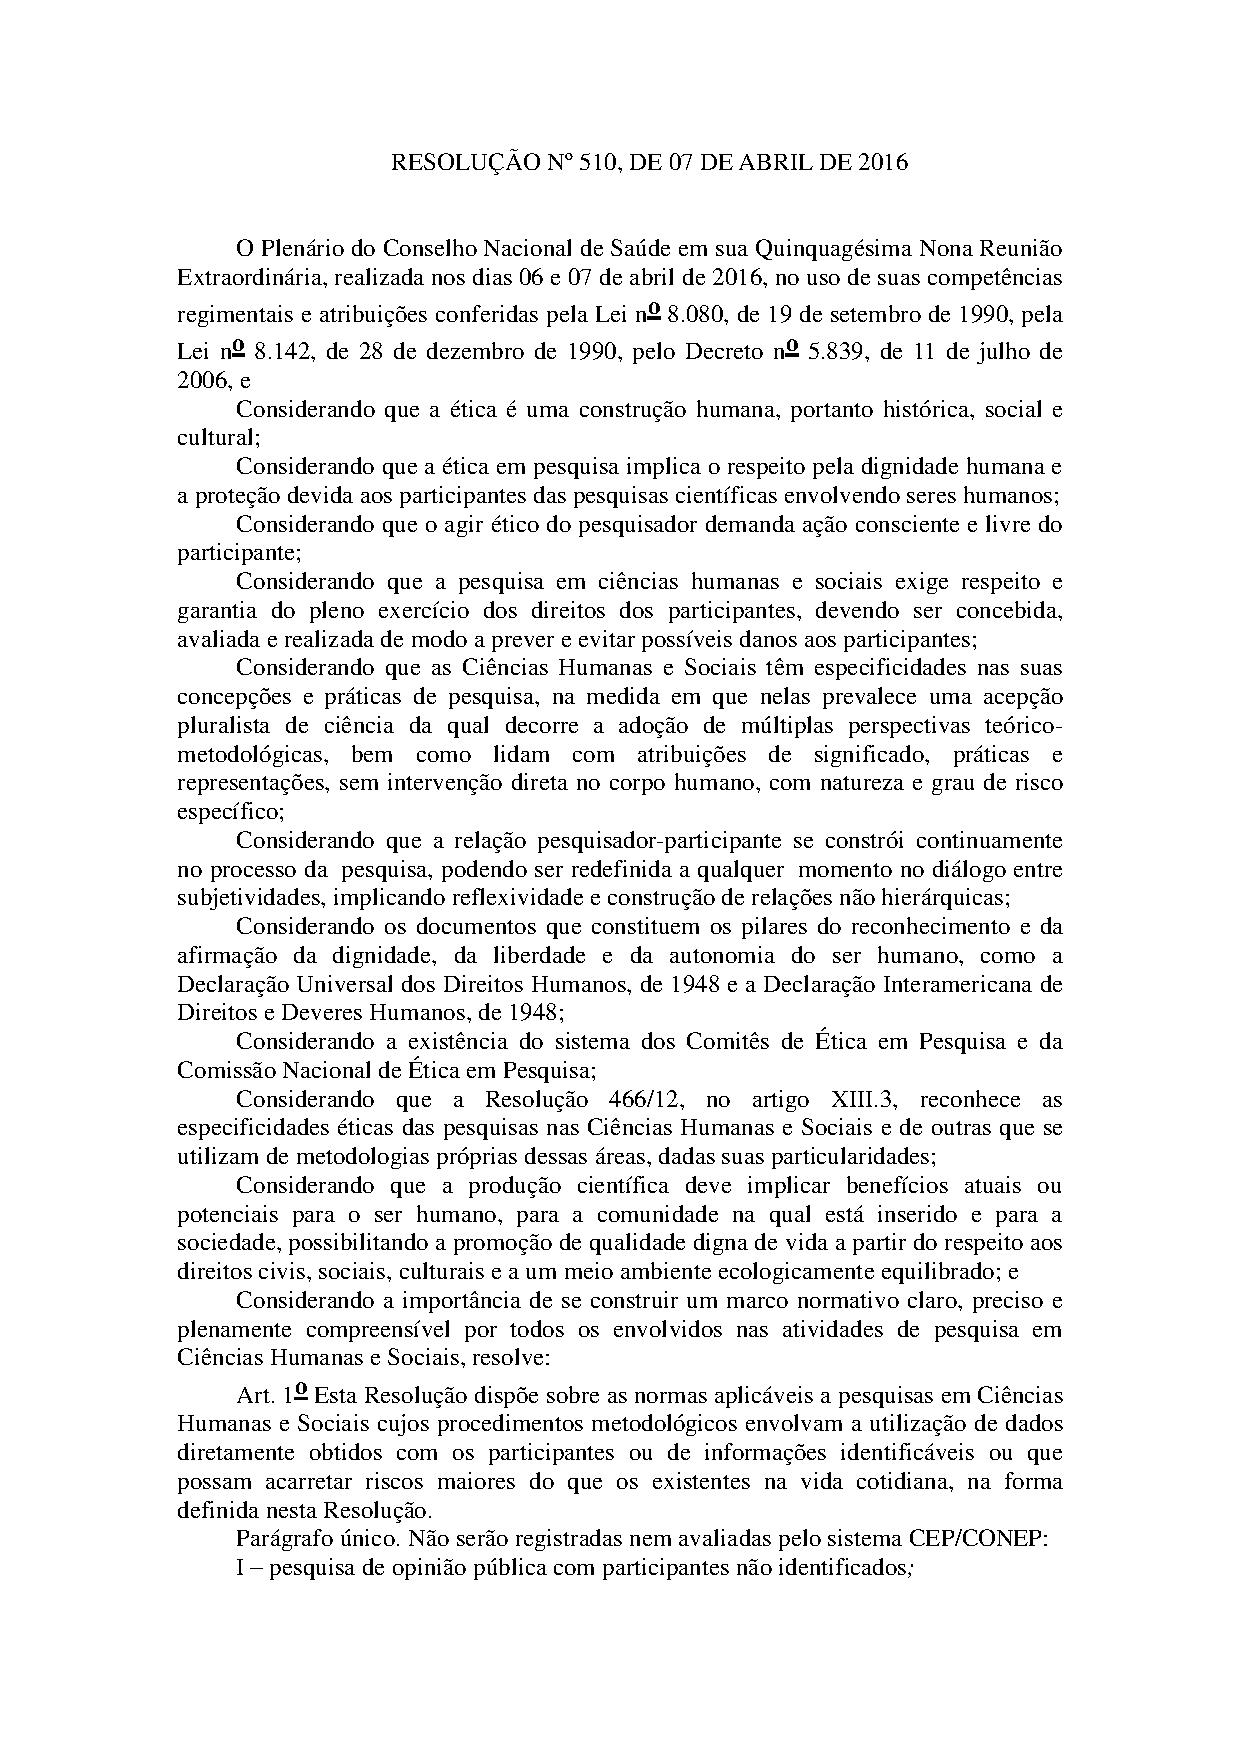
\includepdf[pages=1, scale=0.85, pagecommand={\chapter{Resolução CNS nº 510, de 7 de abril de 2016}\label{anexo:res510}}]{anexos/resolucao_cns_510_2016.pdf}
\includepdf[pages=2-, scale=0.85, pagecommand={}]{anexos/resolucao_cns_510_2016.pdf}

	% ----------------------------------------------------------
% Anexo B: Resolução CNS nº 466/2012, citada nas Considerações Éticas
% ----------------------------------------------------------
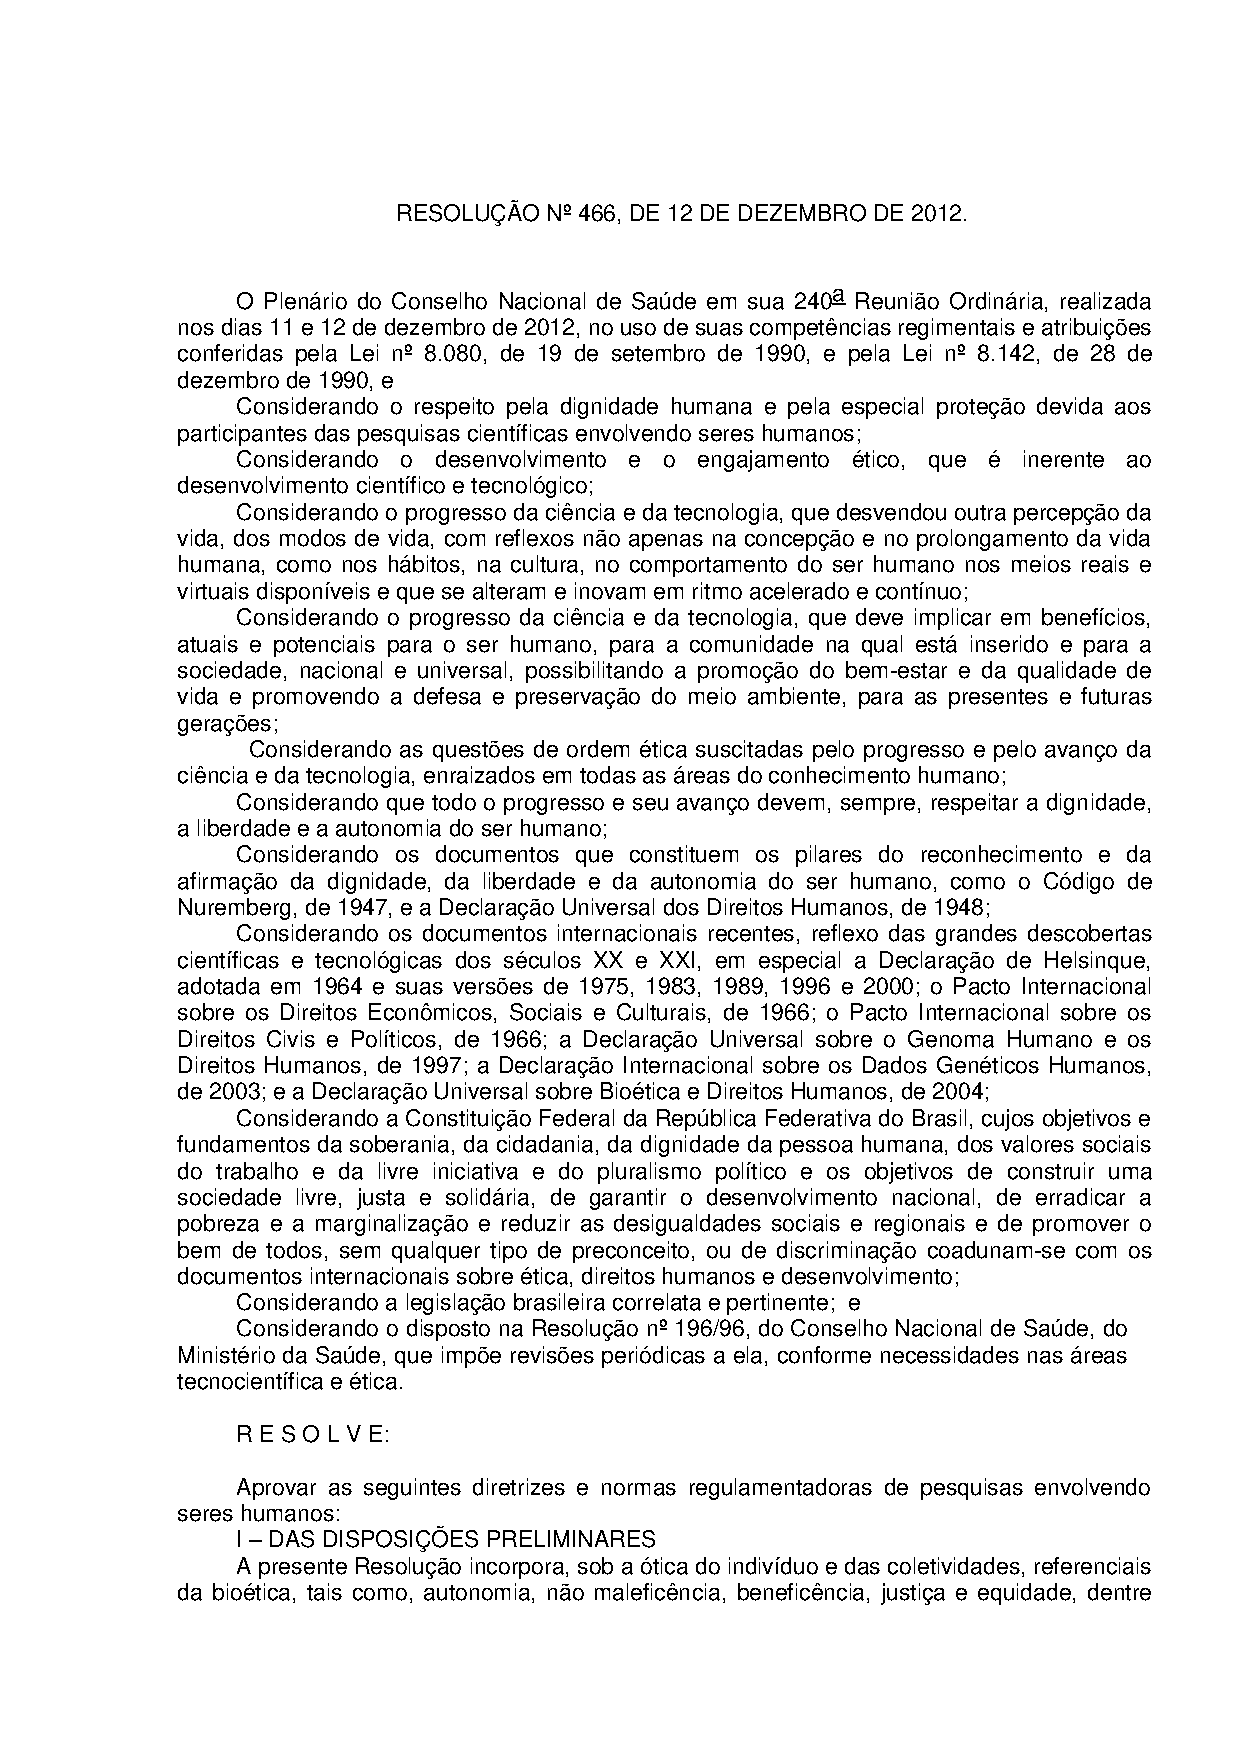
\includepdf[pages=1, scale=0.85, pagecommand={\chapter{Resolução CNS nº 466, de 12 de dezembro de 2012}\label{anexo:res466}}]{anexos/resolucao_cns_466_2012.pdf}
\includepdf[pages=2-, scale=0.85, pagecommand={}]{anexos/resolucao_cns_466_2012.pdf}

\end{anexosenv}

%---------------------------------------------------------------------
% INDICE REMISSIVO
%---------------------------------------------------------------------
%\phantompart
%\printindex
%---------------------------------------------------------------------

\end{document}
